
%% using aastex version 6
\documentclass[twocolumn]{aastex6}

% These are the available options:
%   manuscript	: onecolumn, doublespace, 12pt fonts
%   preprint	: onecolumn, single space, 10pt fonts
%   preprint2	: twocolumn, single space, 10pt fonts
%   twocolumn	: a two column article. Probably not needed, but here just in case.
%   onecolumn	: a one column article; default option.
%   twocolappendix: make 2 column appendix
%   onecolappendix: make 1 column appendix is the default. 
%   astrosymb	: Loads Astrosymb font and define \astrocommands. 
%   tighten	: Makes baselineskip slightly smaller
%   times	: uses times font instead of the default
%   linenumbers	: turn on lineno package.
%   trackchanges : required to see the revision mark up and print output
%   numberedappendix: Labels appendix sections A, B, ... This is the default.
%   appendixfloats: Needed. Resets figure and table counters to zero

\usepackage{verbatim}
\usepackage{amsmath}
\usepackage{graphicx}
\usepackage{cleveref}
\usepackage{hyperref}
\usepackage{multirow}
\usepackage[normalem]{ulem}


\usepackage{xcolor}

\newcommand{\vdag}{(v)^\dagger}
\newcommand\aastex{AAS\TeX}
\newcommand\latex{La\TeX}
\newcommand{\rr}[1]{$r_{#1}$}
\newcommand{\M}[1]{$M_{\mathrm{#1}}$}
\newcommand{\A}{\textit{A}}
\newcommand{\N}{\textit{N}}
\newcommand{\Pf}{$P_{F,0}$}
\newcommand{\Pn}{$P_{N,0}$}
\newcommand{\p}{$p_0$}
\newcommand{\tf}{$t_F$}
\newcommand{\tn}{$t_N$}
\newcommand{\feat}{`Featured'}
\newcommand{\notfeat}{`Not'}
\newcommand{\raw}{GZ2$_{\text{raw}}$}
\newcommand{\deb}{GZ2$_{\text{debiased}}$}
\newcommand{\pmachine}{$p_{\mathrm{machine}}$}
\newcommand{\ffeat}{$f_{\mathrm{featured}}$}
\newcommand{\fsmooth}{$f_{\mathrm{smooth}}$}
\newcommand{\fstar}{$f_{\mathrm{artifact}}$}



%%%%%%%%%%%%%%%%%%%%%%%%%%%%%%%%%%%%%%%%%%%%%%%%%%%%%%%%%%%%%%
%% The following commented section outlines numerous optional output that
%% can be displayed in the front matter or as running meta-data.
%%
%% You can insert a short comment on the title page using the command below.
%% \slugcomment{Not to appear in Nonlearned J., 45.}
%%
%% If you wish, you may supply running head information, although
%% this information may be modified by the editorial offices.
%%
%% You can add a light gray and diagonal water-mark to the first page 
%% with this command:
%% \watermark{text}
%% where "text", e.g. DRAFT, is the text to appear.  If the text is 
%% long you can control the water-mark size with:
%% \setwatermarkfontsize{dimension}
%% where dimension is any recognized LaTeX dimension, e.g. pt, in, etc.
%%
%%%%%%%%%%%%%%%%%%%%%%%%%%%%%%%%%%%%%%%%%%%%%%%%%%%%%%%%%%%%%%%%%%%


\shorttitle{Human and machine morphology classifications}
\shortauthors{Beck et al.}

\begin{document}


\title{Integrating human and machine intelligence in galaxy morphology \\classification tasks}

%% Use \author, \affil, plus the \and command to format author and affiliation 
%% information.  If done correctly the peer review system will be able to
%% automatically put the author and affiliation information from the manuscript
%% and save the corresponding author the trouble of entering it by hand.
%%
%% The \affil should be used to document primary affiliations and the
%% \altaffil should be used for secondary affiliations, titles, or email.

%% Authors with the same affiliation can be grouped in a single
%% \author and \affil call.

\author{Melanie Beck\altaffilmark{1}, Claudia Scarlata\altaffilmark{1}, Lucy F. Fortson\altaffilmark{1}}
\author{Chris J. Lintott\altaffilmark{2, 3}}
\author{Melanie A. Galloway\altaffilmark{1}, Kyle W. Willett\altaffilmark{1}}
\author{B. D. Simmons\altaffilmark{2,4,7}}
\author{Hugh Dickinson\altaffilmark{1}}
\author{Karen L. Masters\altaffilmark{5}}
\author{Philip J. Marshall\altaffilmark{6}}
\author{Darryl Wright\altaffilmark{2}}

%\email{beck@astro.umn.edu}

\altaffiltext{1}{Minnesota Institute for Astrophysics, University of Minnesota, Minneapolis, MN 55455, USA; beck@astro.umn.edu}
\altaffiltext{2}{Oxford Astrophysics, Denys Wilkinson Building, Keble Road, Oxford OX1 3RH, UK}
\altaffiltext{3}{New College, Oxford OX1 3BN, UK}
\altaffiltext{4}{Center for Astrophysics and Space Sciences, Department of Physics, University of California, San Diego, CA 92093, USA}
\altaffiltext{5}{Institute of Cosmology and Gravitation, University of Portsmouth, Portsmouth, UK}
\altaffiltext{6}{Kavli Institute for Particle Astrophysics and Cosmology, P.O. Box 20450, MS29, Stanford, CA 94309, U.S.A.}
\altaffiltext{7}{Einstein Fellow}



\begin{abstract}
Quantifying galaxy morphology is a challenging yet scientifically rewarding task. 
As the scale of data continues to increase with upcoming surveys, traditional 
classification methods will struggle to handle the load. We present a solution through an 
integration of visual and automated classifications, 
preserving the best features of both human and machine. 
We demonstrate the effectiveness of such a system through a re-analysis of visual 
galaxy morphology classifications collected during the Galaxy Zoo 2 (GZ2) project, 
reprocessed with a classification aggregation algorithm dubbed SWAP, 
originally developed for the Space Warps gravitational lens project. 
Incorporating the SWAP algorithm increases the classification rate by a factor of 4.7, 
classifying 226,124 galaxies in 92 days of GZ2 project time. GZ2 classified  $\sim$$48$K in the same time period. This increased rate does not diminish the quality of classification as we 
maintain 95.7\% accuracy when compared to GZ2 published data. 
We next combine this with a Random Forest machine learning algorithm that 
learns on a suite of non-parametric morphology indicators widely used for automated morphologies.
We develop a decision engine that delegates tasks between human and machine, and
demonstrate that the combined system provides a factor of 11.4 increase in the classification rate, 
classifying 210,543 galaxies in just 32 days of GZ2 project time. 
Again, this impressive performance is achieved with 93.5\% accuracy. 
As the Random Forest algorithm requires a minimal amount of computational cost, 
this result has important implications for galaxy morphology 
identification tasks in the era of \textit{Euclid} and other large-scale surveys.
\end{abstract}


%% Keywords should appear after the \end{abstract} command. 
%% See the online documentation for the full list of available subject
%% keywords and the rules for their use.
\keywords{galaxies: general --- galaxies: morphology  --- methods: data analysis --- methods: machine learning}


\section{Introduction} \label{sec:intro}

Astronomers have made use of visual galaxy morphologies to understand the dynamical structure of these systems for nearly ninety years 
\citep[e.g.,][]{Hubble1936, 
			deVauc1959, 
			Sandage1961, 
			vandenBergh1976, 
			NairAbraham2010, 
			Baillard2011}. 
The division between early-type and late-type systems corresponds, for example, to a wide range of parameters from mass and luminosity, to environment, color, and star formation history 
\citep[e.g.,][]{Kormendy1977,  
			Dressler1980, 
			Strateva2001, 
			Blanton2003, 
			Kauffman2003, 
			Nakamura2003, 
			Shen2003, 
			Peng2010}; 
while detailed observations of morphological features such as bars and bulges 
provide information about the history of their host systems 
\citep[e.g., review by][]{KK04, 
			Elmegreen2008, 
			Sheth2008, 
			Masters2010, 
			Simmons2014}. 
Modern studies of morphology  divide systems into broad classes 
\citep[e.g.,][]{Conselice2006, 
			Lintott2008, 
			Kartaltepe2015, 
			Peth2016}, 
but a wealth of information can be gained from identifying new and often rare classes, 
such as low redshift clumpy galaxies \citep[e.g.,][]{Elmegreen2013}, polar-ring galaxies \citep[e.g.,][]{Whitmore1990}, and the green peas \citep{Cardamone2009}. 


While the Galaxy Zoo project has provided a solution that scales visual classification 
for current surveys \citep{Lintott2008, Lintott2011, Willett2013, Willett2017, Simmons2017}, 
producing a prolific amount of scientific output \citep[e.g.,][]{Land2008, Bamford2009, Darg2010, Schawinski2014, Galloway2015, Smethurst2016}, 
upcoming surveys such as \textit{LSST} and \textit{Euclid}
will require a different approach, imaging more than a billion new galaxies  \citep{LSST, Euclid}. 
If detailed morphologies can be extracted for just  0.1\% of this imaging, we will 
have millions of images to contend with. A project of this magnitude would take more than 
sixty years to classify at Galaxy Zoo's current rate and configuration. Standard visual morphology     
methods will thus be unable to cope with the scale of data. 

Another approach has been the use of automated morphologies with the development
of parametric \citep{Sersic1968, Odewahn2002, Peng2002}, 
and non-parametric \citep{Abraham1994, Conselice2003, Abraham2003, Lotz2004, Freeman2013} 
structural indicators. While these scale well to large samples 
\citep[e.g.,][]{	Simard2011, 
			Griffith2012, 
			Casteels2014, 
			Holwerda2014, 
			Meert2016}, 
they often fail to capture detailed structure and can 
provide only statistical morphologies with large uncertainties \cite[e.g.,][]{Abraham1996, Bershady2000}. 


%%%-------------------------------------------------------
%%% FIGURE:     GZ EXPRESS Schematic
%%%-------------------------------------------------------
\begin{figure*}[ht!]
%\figurenum{1}
\plotone{figures/GZExpress_v4.pdf}
\caption{Schematic of our hybrid system. Humans provide classifications of galaxy images via a web interface. We simulate this with the Galaxy Zoo 2 classification data described in Section~\ref{sec: data}. Human classifications are processed with an algorithm described in Section~\ref{sec: SWAP}. Subjects that pass a set of thresholds are considered human-retired (fully classified) and provide the training sample for the machine classifier as described in Section~\ref{sec: machine}. The trained machine is applied to all subjects not yet retired. Those that pass an analogous set of machine-specific thresholds are considered machine-retired. The rest remain in the system to be classified by either human or machine. This procedure is repeated  nightly. Our results are reported in Section~\ref{sec: results}.  \label{fig: schematic}}
\end{figure*}

Machine learning techniques are becoming increasingly popular for classification 
and image processing tasks. Another automated approach, these generally work
by defining a set of features that describe the morphology in an $N$-dimensional space. 
The location in this morphology space defines a morphological type for each galaxy.
Learning the morphology space can be achieved through algorithms such as 
Support Vector Machines \citep{HuertasCompany2008} 
or Principal Component Analysis \citep{Watanabe1985, Scarlata2007}.  
Another approach is through deep learning, a machine learning technique that attempts 
to model high level abstractions. Algorithms like convolutional and artificial 
neural networks (CNNs, ANNs) have been used for galaxy morphology classification 
with impressive accuracy 
\citep{Ball2004, 
	Banerji2010, 
	Dieleman2015, 
	HuertasCompany2015}. 
A drawback to all machine learning classification techniques is the need for 
standardized training data, with more complex algorithms requiring more data. 
Furthermore, that data must be consistent for each survey: differences in resolution 
and depth can be inherently learned by the algorithm making their application to 
disparate surveys challenging.  


In this work we present a system that preserves the best features of both visual and 
automatic classifications, developing for the first time a framework that brings both 
human and machine intelligence to the task of galaxy morphology to handle the 
scale and scope of next generation data. We demonstrate the effectiveness of such 
a system through a re-analysis of visual galaxy morphology classifications collected 
during the Galaxy Zoo 2 project, and combine these with a Random Forest
machine learning algorithm that trains on a suite of non-parametric morphology 
indicators widely used for automated morphologies. 
Our method provides a factor of 11.4 increase in the rate of galaxy morphology
classification, and a factor of 10 reduction in human effort, while maintaining 
at least 93.5\% classification accuracy as compared to Galaxy Zoo 2 published data. 
We first present an overview of our framework, which also serves as a blueprint for this paper. 


%%----------------------------------------------------------------------------------------------------------------------------------------------------
%%   GALAXY ZOO EXPRESS OVERVIEW
%%---------------------------------------------------------------------------------------------------------------------------------------------------
\section{Galaxy Zoo Express Overview}

The Galaxy Zoo Express (GZX) framework combines human and machine to 
increase morphological classification efficiency, both in terms of the 
classification rate and required human effort. 
Figure~\ref{fig: schematic} presents a schematic of GZX including section 
numbers as a shortcut for the reader. We note that transparent portions
 of the schematic represent areas of future work which we explore in Section~\ref{sec: visions}. 
Any system combining human and machine classifications will have a set of generic 
features: a group of human classifiers, at least one machine classifier, and a 
decision engine which determines how these classifications should be combined.

In this work we demonstrate our system through a re-analysis of  Galaxy Zoo 2 (GZ2) classifications. 
This allows us to  create simulations of human classifiers (described in Section~\ref{sec: data}).
These classifications are used most effectively when processed with SWAP, 
a Bayesian code described in Section~\ref{sec: SWAP}, first developed for the 
Space Warps gravitational lens discovery project~\citep{Marshall2016}. 
These subjects provide the machine's training sample. 

In Section~\ref{sec: machine}, we incorporate a machine classifier. We have 
developed a Random Forest algorithm that trains on measured morphology
indicators such as Concentration, Asymmetry, Gini coefficient and \M{20}. 
After a sufficient number of subjects have been classified by humans, 
 the machine is trained and its performance assessed through cross-validation. 
This procedure is repeated nightly and the machine's performance increases with
size of the training sample, albeit with a performance limit. 
Once the machine reaches an acceptable level of 
performance it is applied to the remaining galaxy sample. 


Even with this simple description, one can see that the classification process 
will progress in three phases.  First, the machine will not yet have reached an 
acceptable level of performance; only humans contribute to subject classification.
Second, the machine's performance will improve; both humans and machine 
will be responsible for classification. Finally, machine performance 
will slow; remaining images will likely need to be classified by humans. 
These results are explored in  Section~\ref{sec: results}. 
This blueprint allows even modest machine learning 
routines to make significant contributions alongside human classifiers and 
removes the need for ever-increasing performance in machine classification.



%%----------------------------------------------------------------------------------------------------------------------------------------------------
%%   Galaxy Zoo 2 Data Description
%%---------------------------------------------------------------------------------------------------------------------------------------------------
\section{Galaxy Zoo 2 Classification Data} \label{sec: data}

Our simulations utilize original classifications made by volunteers during the GZ2 project. 
These data\footnote{\url{data.galaxyzoo.org}} are described in detail in~\cite{Willett2013}, 
though we provide a brief overview here.  
The GZ2 subject sample consists of 285,962 galaxies identified as the
 brightest 25\% ($r$-band magnitude $< 17$) residing in the SDSS North Galactic 
Cap region from Data Release 7 and included subjects with both spectroscopic and 
photometric redshifts out to $z < 0.25$,


Subjects were shown as color composite images via a web-based interface\footnote{\url{www.galaxyzoo.org}} wherein 
volunteers answered a series of questions pertaining to the morphology of the subject.
With the exception of the first question, subsequent queries were 
dependent on volunteer responses from the previous task creating a complex decision tree. 
Using GZ2 nomenclature,  a \textit{classification} is the total amount of
information about a subject obtained by completing all tasks in the decision tree. 
A subject is \textit{retired} after it has achieved a sufficient number of classifications.
%\footnote{\url{zoo2.galaxyzoo.org}}


For our current analysis, we choose the first task in the tree: 
``Is the galaxy simply smooth and rounded, with no sign of a disk?" to which possible 
responses include ``smooth", ``features or disk", or ``star or artifact". 
This serves two purposes: 1) this is one of only two questions in the GZ2
decision tree that is asked of every subject, thus maximizing the amount of data
we have to work with, and 2) our analysis assumes a binary task and this question is 
simple enough to cast as such. 

By combining the ``star or artifact" vote fraction, $f_{artifact}$, 
with the ``features or disk" vote fraction, $f_{features}$ we obtain a binary response.
Here, a vote fraction is simply the fraction of volunteers who voted for a
particular response.  
We define a label for each GZ2 subject as the majority vote fraction, that is,
if \ffeat+\fstar~$ >$ \fsmooth, the galaxy is labeled~\feat, otherwise
it is labeled~\notfeat. 
We note that only 512 subjects in the GZ2 catalog have a majority \fstar, 
contributing less than half a percent contamination.

The GZ2 catalog assigns every subject three types of volunteer vote fractions: 
raw, weighted, and debiased. 
Debiased vote fractions are calculated to correct for redshift bias, a task that 
GZX does not perform. 
The weighted vote fractions account for inconsistent volunteers, 
a task we perform as well. However, because our mechanism is entirely different 
from GZ2, we derive labels from the raw vote fractions (\raw).
 In total, the data consist of over 16 million classifications from 83,943 individual volunteers. 


%%----------------------------------------------------------------------------------------------------------------------------------------------------
%%   Talk About SWAP 
%%----------------------------------------------------------------------------------------------------------------------------------------------------
\section{Efficiency through intelligent human-vote aggregation}\label{sec: SWAP}

Galaxy Zoo 2 had a brute-force subject retirement rule whereby each galaxy 
was to receive approximately forty independent classifications. 
Once the project reached completion, inconsistent volunteers were down-weighted~\citep{Willett2013}, 
a process that does not make efficient use of those who are exceptionally skilled. 
To intelligently manage subject retirement and increase classification efficiency, 
we adapt an algorithm from the Zooniverse project Space Warps~\citep{Marshall2016}, 
which searched for and discovered several gravitational lens candidates in the 
CFHT Legacy Survey~\citep{More2016}.  
Dubbed SWAP (Space Warps Analysis Pipeline),  this algorithm predicted the 
probability that an image contained a gravitational lens given 
volunteers' classifications and experience after being shown a training
sample consisting of simulated lensing events.  We provide a brief overview here.  

The algorithm assigns each volunteer an \textit{agent} which interprets that volunteer's 
classifications. Each agent assigns a 2$\times$2 confusion matrix to their volunteer which encodes
that volunteer's probability of correctly identifying feature `\A',  given that the subject 
actually exhibits feature \A; and the probability of correctly identifying
the absence of feature \A, given that the subject does not exhibit 
that feature. The agent updates these probabilities by estimating them as 
\begin{equation}
P(``X" | X, d) \approx \frac{N_{``X"}}{N_{X}}
\end{equation}
where $N_{``X"}$ is the number of classifications the volunteer labeled as type $X$, 
$N_X$ is the number of subjects the volunteer has seen that were actually of type $X$,
and $d$ represents the history of the volunteer, i.e., all subjects they have seen. 


Each subject is assigned a prior probability that it exhibits feature \A: $P(A) = p_0$. 
When a volunteer makes a classification, Bayes' theorem is used to derive how 
that subject's prior probability should be updated into a posterior using elements
of the agent's confusion matrix. 
As the project progresses, each subject's probability is continually updated,
 nudged higher or lower depending on volunteer input.
Probability thresholds can be set such that subjects crossing a threshold
are highly likely to exhibit the feature of interest or the absence thereof. 
These subjects are then considered retired. 


%% -------------------------------------------------------------------------------
%%   FIGURE:  VOLUNTEER PROBABILITIES
%% -------------------------------------------------------------------------------
\begin{figure}[t!]
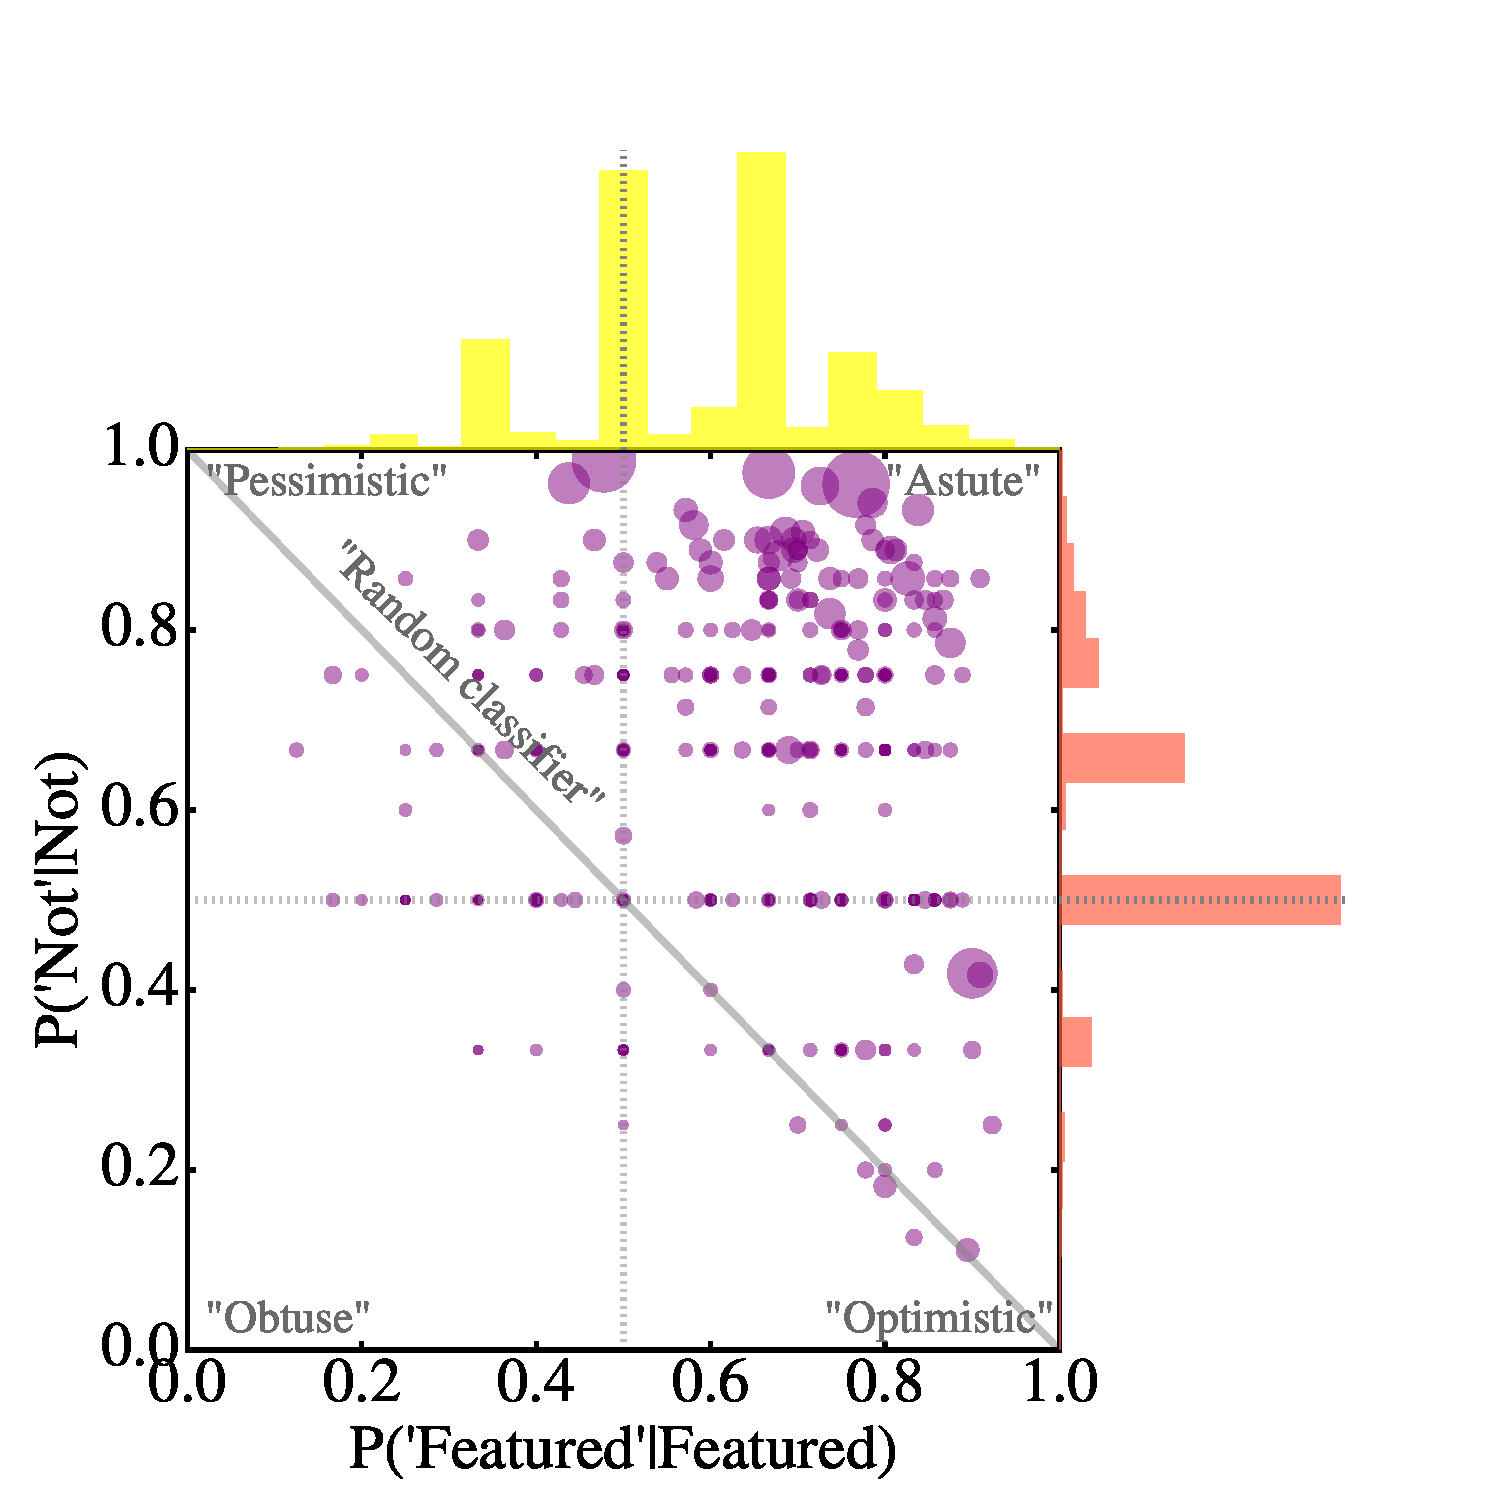
\includegraphics[width=3.7in]{figures/volunteer_confusion_matrix.pdf}
\caption{Confusion matrices for 1000 randomly selected GZ2 volunteers after fiducial SWAP assessment. Circle size is proportional to the number of gold standard subjects that volunteer classified. The histograms on top and right represent the distribution of each component of the confusion matrix for all volunteers.  A quarter of GZ2 volunteers are ``Astute"; they are adept at correctly identifying both~\feat~and~\notfeat~subjects. The peaks at 0.5 in both distributions are due to volunteers who see only one training image; only half of their confusion matrix is updated. \label{fig: volunteer training}}
\end{figure}

\subsection{Volunteer Training Sample}\label{sec: training sample}

A key feature of the original Space Warps project was the training of 
individual volunteers through the use of simulated images.
These were interspersed with real imaging and were 
predominantly shown at the beginning of a volunteer's association with the project, 
allowing that volunteer's agent time to update before classifying real data. 
Volunteers were provided feedback in the form of a pop-up comment after
classifying a training image. GZ2 did not train volunteers in such a way, which
presents a challenge when applying SWAP to GZ2 classifications. 
We describe how we engineer the GZ2 data to mimic the Space 
Warps system.


We create a gold standard sample by selecting 3496 SDSS galaxies 
representative of the relative abundance of T-Types, a numerical index of a galaxy's stage along 
the Hubble sequence, at $z\sim0$ by considering galaxies that overlap 
with the~\cite{NairAbraham2010} catalog, a collection of $\sim$14K galaxies 
classified by eye into T-Types. 
Expert classifications were obtained through the Zooniverse platform\footnote{The Project Builder template facility can be found at \url{http://www.zooniverse.org/lab.}}  
from 15 professional astronomers, including members of the Galaxy Zoo science team. 
 The question posed was identical to the original GZ2 question and at least five 
experts classified each galaxy. 
Votes are aggregated and a simple majority provides an expert label for each subject. 
Our final dataset consists of the GZ2 classifications made 
by those volunteers who classify at least one of these gold standard subjects. 
We thus retain for our simulation 12,686,170 classifications from 30,894 unique volunteers. 
Classifications of gold standard subjects are always processed first. 



%%%-------------------------------------------------------
%%%  FIGURE:    SWAP FIDUCIAL RUN
%%%-------------------------------------------------------
\begin{figure}[t!]
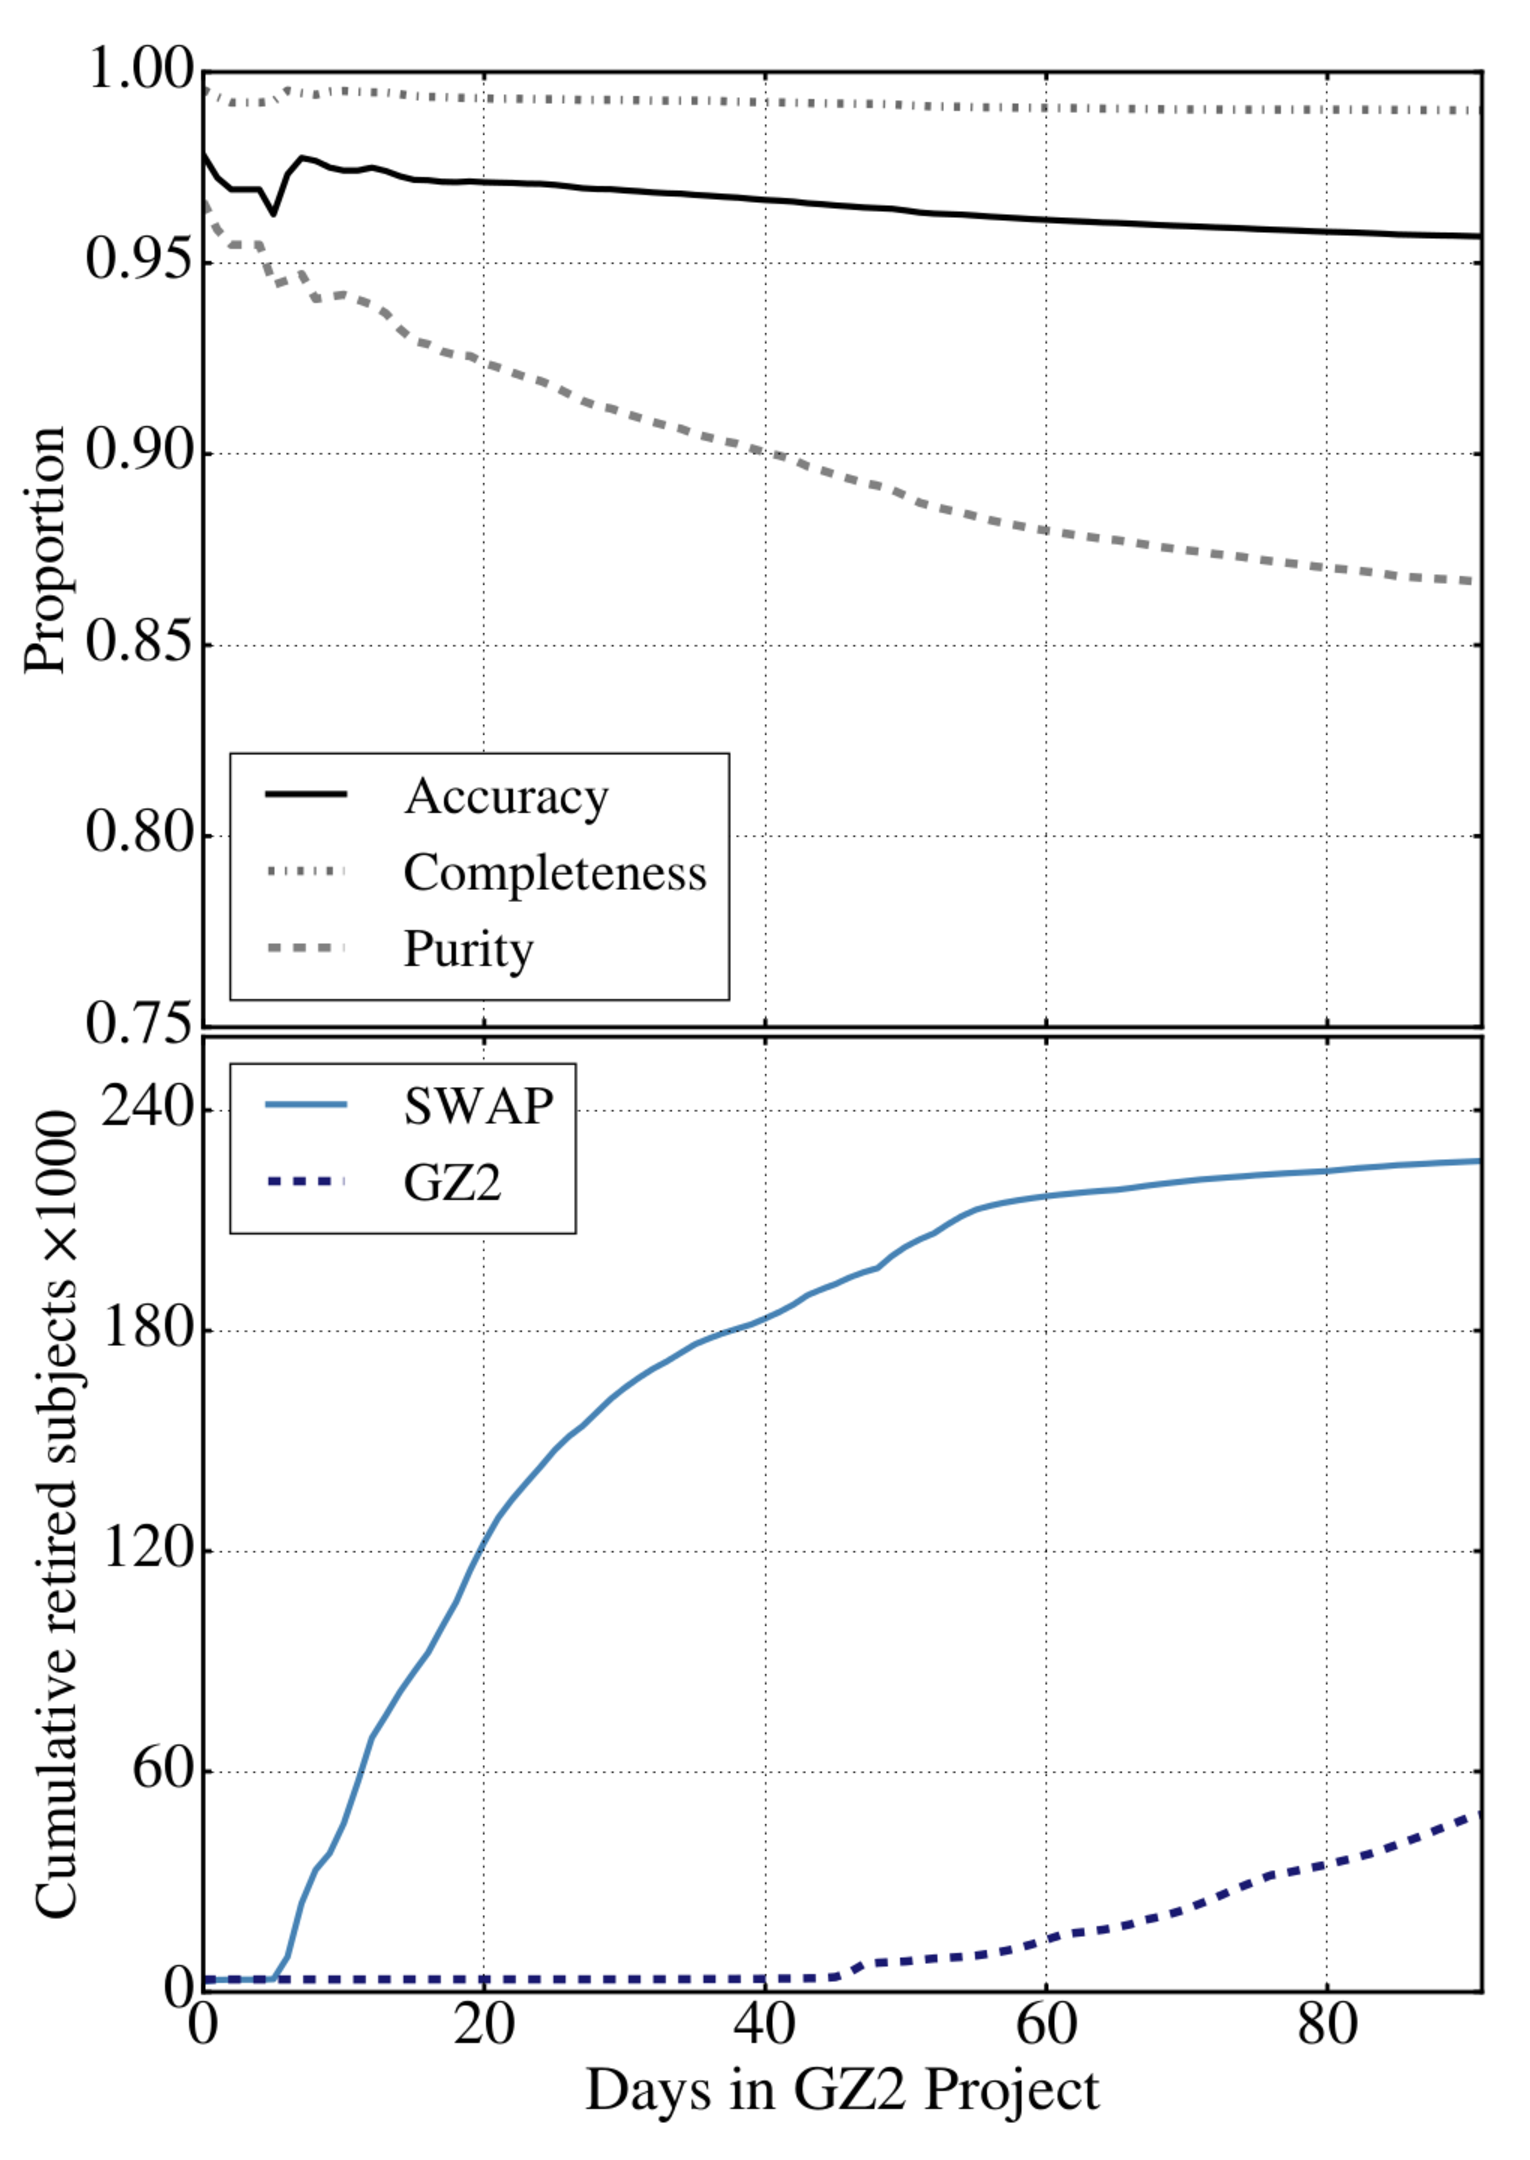
\includegraphics[width=3.35in]{figures/GZX_eval_and_retirement_baseline_4paper.pdf}
\caption{Fiducial SWAP simulation demonstrates a factor of 4-5 increase in the rate of subject retirement as a function of GZ2 project time (bottom panel, light blue) compared with the original GZ2 project (dashed dark blue). After 92 days, SWAP retires over 225K subjects, while GZ2 retires $\sim$48K.  The top panel displays the quality metrics (greys). These are calculated by comparing SWAP-assigned labels to~\raw~labels (Section~\ref{sec: data}) for the subject sample retired by that day of the simulation. Thus, on the final day, SWAP retires 226,124 subjects with 95.7\% accuracy,  and with completeness and purity of~\feat~subjects at 99\% and 86.7\% respectively. The decrease in purity as a function of time is due, in part, to the fact that more difficult to classify subjects are retired later in the simulation. 
\label{fig: fiducial run}}
\end{figure}

%%%-------------------------------------------------------
%%%  FIGURE:   SWAP vote distributions
%%%-------------------------------------------------------
\begin{figure}[t!] 
\centering
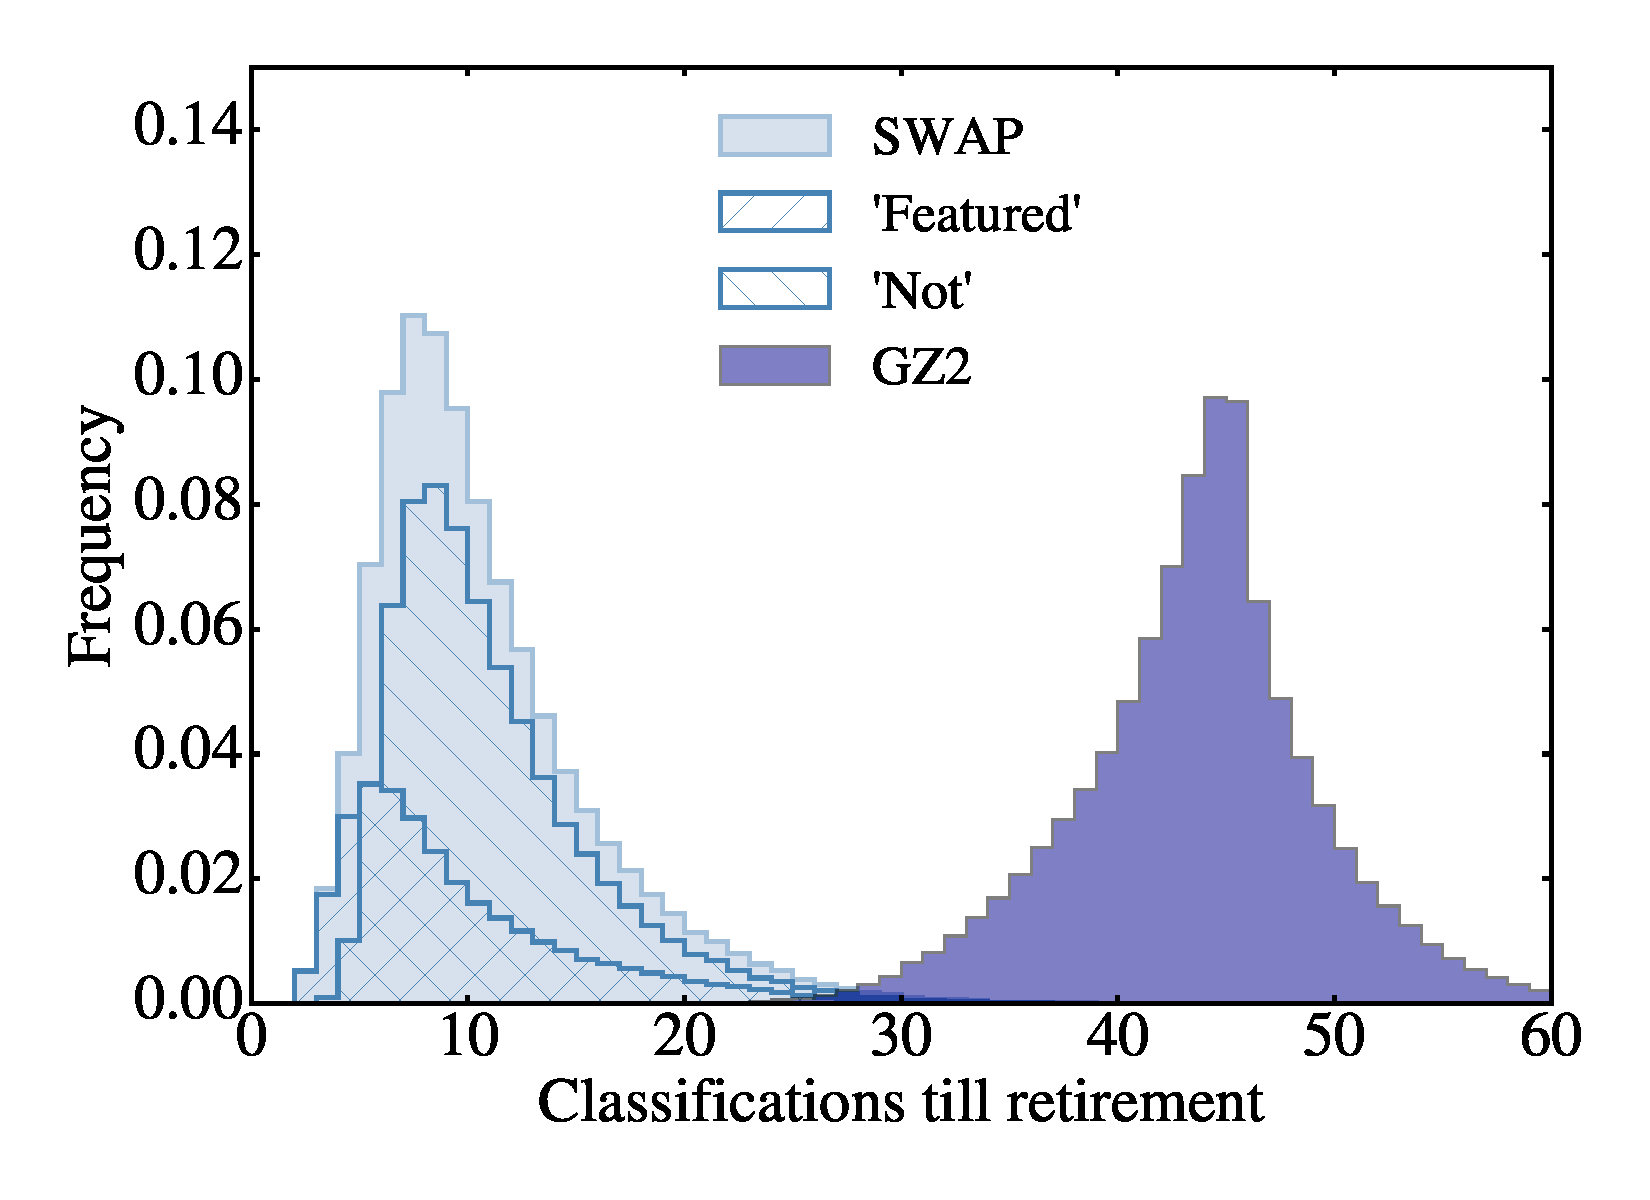
\includegraphics[width=3.5in]{figures/GZX_clicks_till_retired_baseline.pdf}
\caption{SWAP requires 4-5 times less human effort than GZ2 as evidenced by the distribution of the number of classifications a subject requires for retirement for the 226,124 subjects retired during our fiducial run.  The GZ2 distribution peaks around 45 classifications per subject with 98.6\% having at least 30 volunteer votes. In contrast, most subjects need only 9 classifications when processing with SWAP.  Furthermore,  `easy' subjects can reach retirement in as few as 3-4 classifications. \label{fig: swap vote distributions}}
\end{figure}


%%----------------------------------------------------------------------------------------------------------------------------------------------------
%%   Subsection:    		SWAP only (FIDUCIAL RUN)
%%----------------------------------------------------------------------------------------------------------------------------------------------------
\subsection{Fiducial SWAP simulation}\label{sec: fiducial}


Before we run a simulation, a number of SWAP parameters must be chosen: 
 the initial confusion matrix for each volunteer's agent, the subject 
prior probability, and the retirement thresholds. 
For our fiducial  simulation, we initialize all confusion matrices at (0.5, 0.5), 
and set the subject prior probability, \p~$= 0.5$. 
We set the~\feat~threshold, \tf, i.e., the minimum probability for a subject to be retired as~\feat, to $0.99$. Similarly, we set the~\notfeat~threshold, \tn~$= 0.004$. 
In Appendix~\ref{sec: tweaking swap} 
we show that varying these parameters has only a small affect on the SWAP output. 
To simulate a live project, we run SWAP on a time step of $\Delta t = 1$ day, 
during which SWAP processes all volunteer classifications with timestamps 
within that range. This is performed for three months worth of GZ2 classification data. 

Figure~\ref{fig: volunteer training} (adapted from Figure 4 of~\citealt{Marshall2016})
demonstrates the volunteer assessment we achieve, and shows confusion matrices 
 for 1000 randomly selected volunteers. The circle size is proportional to the number of 
gold standard subjects each volunteer classified. 
The histograms represent the distribution of each component
of the confusion matrix for all volunteers.
 Nearly 25\% of volunteers are considered `Astute'  indicating
they are generally good at correctly identifying both~\feat~and~\notfeat~subjects.
The spikes at $0.5$ in the histograms are due to volunteers who see only one 
gold standard subject (i.e.,~\feat), leaving their probability in the 
other (\notfeat) unchanged.
Additionally, 4\% of volunteers have a confusion matrix of (0.5, 0.5) indicating these 
volunteers classified two gold standard subjects of the same type, one correctly and 
one incorrectly. 

Our goal is to increase the efficiency of galaxy classification. We therefore
 use as a metric the cumulative number of retired subjects
as a function of the original GZ2 project time.
We define a subject as GZ2-retired once it achieves at least 30 volunteer votes, 
encompassing 98.6\% of GZ2 subjects.
In contrast, a subject is considered SWAP-retired once its posterior 
probability crosses either of the retirement thresholds defined above. 

However, it is important not to prioritize efficiency at the expense of quality. 
We thus also consider the metrics of accuracy, 
purity and completeness as a function of GZ2 project time.  These are 
defined as follows: accuracy is the number of correctly
identified subjects divided by the total number retired; completeness is the number of 
correctly identified~\feat~subjects divided by the number of actual~\feat~retired; 
and purity is the number of correctly identified~\feat~subjects divided by 
the number of subjects retired as~\feat. Thus, a complete sample has no false
negatives whereas a pure sample has no false positives. 
We compute these metrics by comparing the SWAP-assigned labels of the cumulatively 
retired subject set to the~\raw~labels for each day of the simulation. 
For example, by Day 20, SWAP retires 120K subjects with 96\% accuracy,
 99.7\% completeness, and 92\% purity. 

Figure \ref{fig: fiducial run} and Table~\ref{tab: summary} detail the results of 
our fiducial SWAP simulation compared to the original GZ2 project. 
The bottom panel shows the cumulative number of retired subjects as a function of 
GZ2 project time. By the end of our simulation, GZ2 (dashed dark blue)
 retires $\sim$50K subjects while SWAP (solid light blue) retires 226,124 subjects.  
We thus classify 80\% of the entire GZ2 sample in three months. 
The original GZ2 project took approximately one year to classify as many subjects, 
representing a factor of four increase in the classification rate.  
The top panel of Figure~\ref{fig: fiducial run} demonstrates the quality of 
those classifications as a function of time and establishes that our full 
SWAP-retired sample is 95.7\% accurate, 99\% complete, and 86.7\% pure.

There is also a reduction in the human effort required to perform this classification task.
  Figure~\ref{fig: swap vote distributions} shows the distribution of the number 
of volunteer classifications per subject achieved through SWAP (light blue) 
and GZ2 (dark blue) for the 226K subjects retired in our fiducial run. 
GZ2's distribution peaks at $\sim$45 indicating that, on average,
45 unique volunteers classify each subject. On the other hand, SWAP's
distribution peaks around 9 classifications per subject. 
Furthermore, subjects that are `easy' to classify (i.e.,~\feat) require
even fewer classifications to reach strong consensus. 
More precisely, SWAP processes $2.3 \times 10^6$ volunteer 
classifications while GZ2 records $\sim$$10^7$ for the same subject set. 
SWAP reduces human effort by more than a factor of four. 



%%%-------------------------------------------------------
%%%  FIGURE:   SWAP failures
%%%-------------------------------------------------------
\begin{figure}[t!]
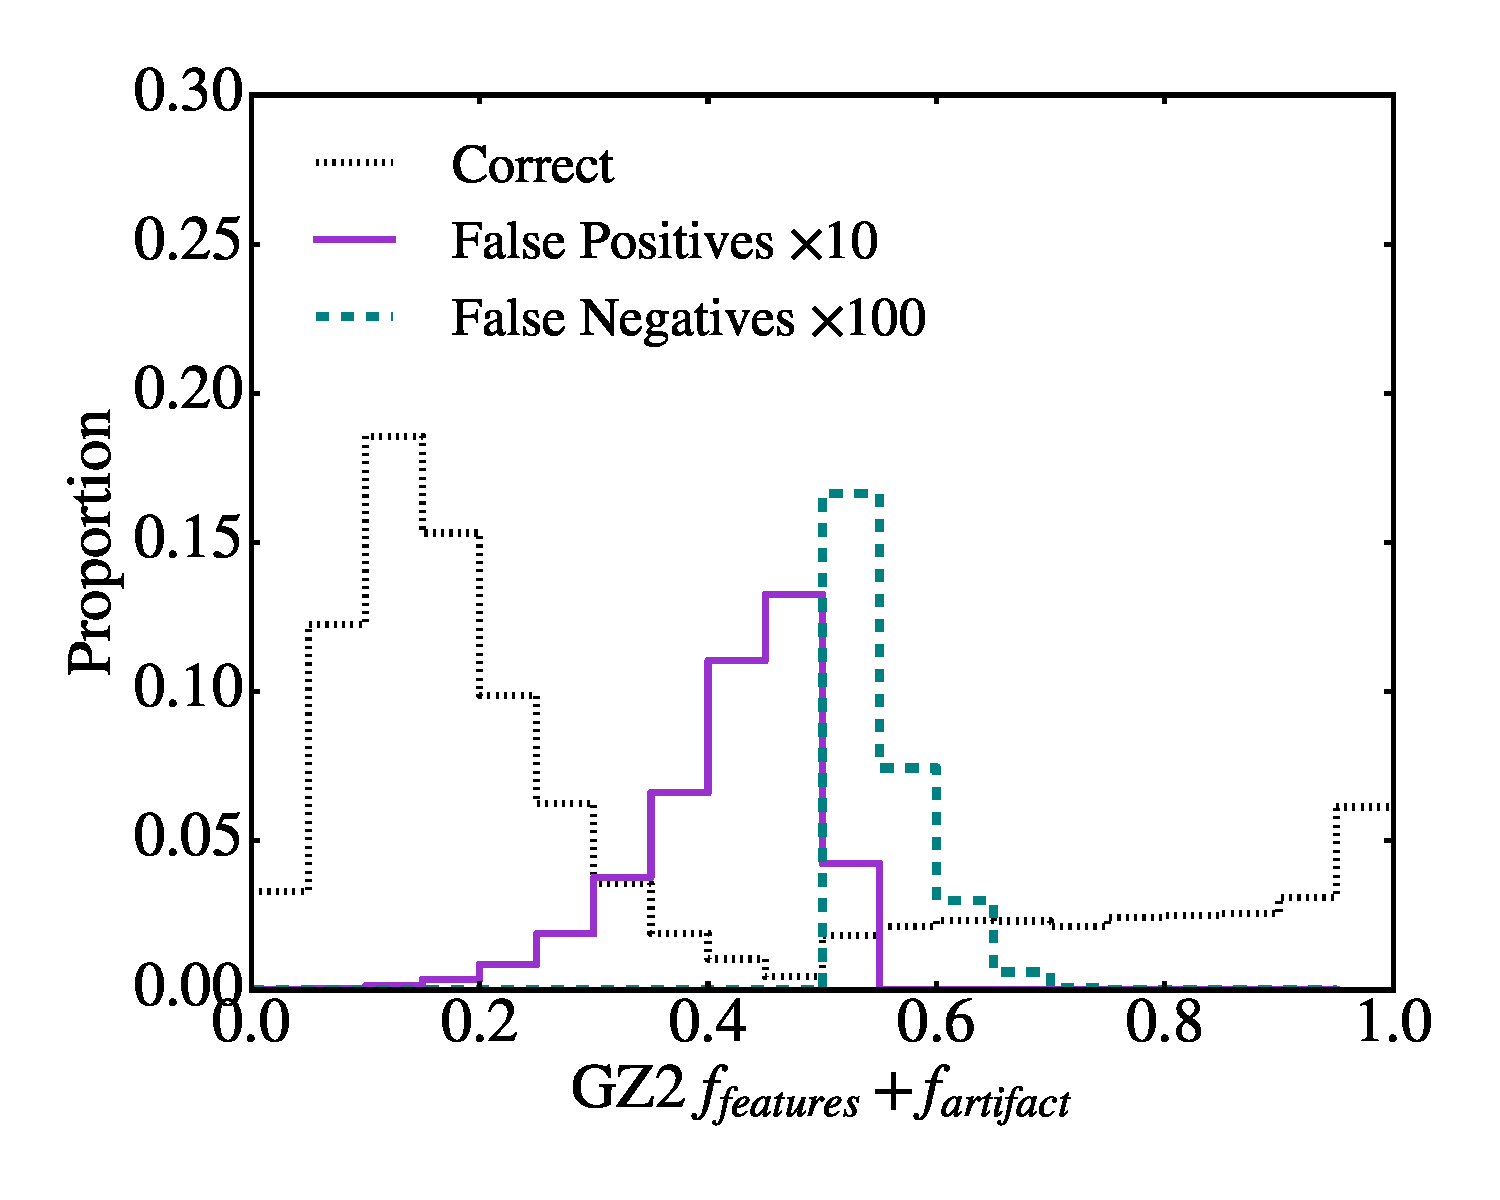
\includegraphics[width=3.5in]{figures/SWAP_GZ2_disagree.pdf}
\caption{Distribution of GZ2 \ffeat+\fstar~vote fractions for subjects correctly identified by SWAP (dotted grey), along with those identified as false positives (solid purple), and false negatives (dashed teal). 
The false positives and false negatives are scaled by factors of 10 and 100 respectively for easier comparison. From Section~\ref{sec: data}, subjects with values $> 0.5$ are defined as~\feat, however, the teal distribution indicates that SWAP labels them as~\notfeat. This is not a flaw of SWAP: 68.9\% of incorrectly identified subjects have $0.4 \le $~\ffeat +\fstar~$ \le 0.6$ suggesting that~\raw~labels are simply too uncertain. The overlap between the false positives and negatives is due to subjects that are exactly 50-50; by default these are labeled~\notfeat. \label{fig: SWAP sucks}}
\end{figure}

As we demonstrate in Appendix~\ref{sec: tweaking swap}, varying the initial SWAP 
parameters from the fiducial values does not substantially change the results 
presented here. The largest influence comes from choosing unrealistic subject 
prior probabilities, which can mildly degrade the quality of the resulting classifications. 
More importantly, none of these effects significantly alters our human and machine integration in Section~\ref{sec: results}. 



\subsection{Disagreements between SWAP and GZ2}
Galaxy Zoo's strength comes from the consensus of dozens of volunteers voting on each subject. 
Processing votes with SWAP reduces the number of classifications to reach consensus. 
Though we typically recover the~\raw~label, SWAP disagrees about 5\% of the time. 
We thus examine the false positives (subjects SWAP labels as~\feat~but~\raw~labels as~\notfeat) and false negatives (subjects SWAP labels as~\notfeat~but~\raw~labels as~\feat).

We find the majority of these disagreements are due to uncertainties in 
the~\raw~label. Figure~\ref{fig: SWAP sucks} shows the distribution of~\ffeat+\fstar~for the false positives (solid purple), and the false negatives (dashed teal) compared to the
majority of subjects wherein SWAP and GZ2 agree (dotted grey).  
Recall that if this value is greater than 0.5, the subject is labeled~\feat.  
The majority of incorrectly 
labeled subjects have $0.4 \le$~\ffeat+\fstar~$\le 0.6$, indicating that 
the GZ2 raw vote fractions are simply too uncertain to provide high quality labels. 
We note that the distribution overlap is due to subjects that do not have a majority;
these are labeled~\notfeat~by default. 

Two other effects contribute to the disagreement between SWAP and GZ2. 
First, as the number of classifications used to retire a galaxy decreases, the 
likelihood of misclassification by random chance increases. 
Second, disagreement arises due to expert-level volunteers whose confusion 
matrices are close to 1.0. These volunteers are essentially more 
strongly weighted, allowing that subject's posterior to cross a retirement threshold
in as few as two classifications. In rare cases, despite training, some expert-level 
volunteers get it wrong. These issues can be mitigated by requiring each subject reach 
a minimum number of classifications before allowing its probability to cross a 
threshold, thus combining the best qualities of GZ2 and SWAP. 




\subsection{Summary}

We demonstrate a factor of four or more increase in 
classification efficiency while maintaining 95\% accuracy, nearly perfect 
completeness of~\feat~subjects, and with a purity that can be controlled by careful 
selection of input parameters to be better than 90\% (see Appendix~\ref{sec: tweaking swap}).
Exploring those subjects wherein SWAP and GZ2 disagree, we conclude that 
the majority of this disagreement stems from uncertainty in~\raw~labels.
We now turn our focus towards incorporating a machine
classifier utilizing these SWAP-retired subjects as a training sample. 


%%----------------------------------------------------------------------------------------------------------------------------------------------------
%%   INTEGRATING MACHINE CLASSIFIERS 
%%----------------------------------------------------------------------------------------------------------------------------------------------------
\section{Efficiency through incorporation of machine classifiers} \label{sec: machine}

We construct the full Galaxy Zoo Express by incorporating supervised 
learning, the machine learning task of inference from labeled training data. 
The training data consist of a set of training examples, and must include
an input feature vector and a desired output label.  Generally speaking,
a supervised learning algorithm analyzes the training data and produces a 
function that can be mapped to new examples. An optimized algorithm will 
correctly determine class labels for unseen data. By processing human classifications 
through SWAP, we obtain a set of binary labels by which we can train a machine 
classifier. We briefly outline the technical details of our machine below,  turning
towards the decision engine we develop in Section~\ref{sec: decision engine}. 



%%----------------------------------------------------------------------------------------------------------------------------------------------------
%%   RANDOM FORESTS
%%----------------------------------------------------------------------------------------------------------------------------------------------------
\subsection{Random Forests}
%Because our task is simple, we choose a simple machine. In particular, 
We use a Random Forest (RF) algorithm~\citep{Breiman2001},  
an ensemble classifier that operates by
 bootstrapping the training data and constructing a multitude of individual decision 
tree algorithms, one for each subsample.  
An individual decision tree works by deciding which of 
the input features best separates the classes. It does this by performing 
splits on the values of the input feature that minimize the classification 
error. These feature splits proceed recursively. Decision trees alone are
 prone to overfitting, precluding them from generalizing 
well to new data. Random Forests mitigate this effect by combining the 
output labels from a multitude of decision trees.  Specifically, we use the 
\texttt{RandomForestClassifier} from the Python module \texttt{scikit-learn}
\citep{scikit-learn}. 


%%----------------------------------------------------------------------------------------------------------------------------------------------------
%%   CROSS-VALIDATION
%%----------------------------------------------------------------------------------------------------------------------------------------------------
\subsection{Grid Search and Cross-validation}
Of fundamental importance is the task of choosing an algorithm's hyperparameters, 
values which determine how the machine learns.   For a RF, key quantities include
 the maximum depth of individual trees (\texttt{max\_depth}), the number of trees
in the forest (\texttt{n\_estimators}), and the number of features to consider when 
looking for the best split (\texttt{max\_features}). 
The goal is to determine which values will optimize 
the machine's performance and thus these values cannot be chosen \textit{a priori}. 
We perform a grid search with $k$-fold cross-validation whereby the 
training sample is split into $k$ subsamples. One subsample is withheld to 
estimate the machine's performance while the remaining data is used to train the machine. 
This is performed $k$ times and the average performance
value is recorded. The entire process is repeated for every combination of the 
 hyperparameters in the grid space and values that optimize the output are chosen. 
In this work we let $k=10$, however, we leave this as an adjustable input parameter.
In the interest of computational speed, we set \texttt{n\_estimators} $=30$ and 
perform the grid search for \texttt{max\_depth} over the range $[5,16]$, and 
\texttt{max\_features} over the range $[\sqrt{D}, D]$,
where $D$ is the number of features in the feature vector, described below.
 

%%----------------------------------------------------------------------------------------------------------------------------------------------------
%%   FEATURE REPRESENTATION AND PRE-PROCESSING
%%----------------------------------------------------------------------------------------------------------------------------------------------------
\subsection{Feature Representation and Pre-Processing}
The feature vector on which the machine learns is composed of $D$ individual 
numeric quantities associated with the subject that the machine uses to discern 
that subject from others in the training sample. 
To segregate~\feat~from~\notfeat, we draw on ZEST \citep{Scarlata2007} and compute
 concentration, asymmetry, Gini coefficient, and M$_{20}$, 
the second-order moment of light for the brightest 20\% of galaxy pixels as
measured from SDSS DR12 $i$-band imaging (see Appendix \ref{sec: measuring morphology}). 
Coupled with SExtractor's measurement of ellipticity \citep{sextractor}, 
we provide the machine with a $D=5$ dimensional morphology parameter space. 
These non-parametric diagnostics have long been used to 
quantify galaxy morphology in an automated fashion \cite[e.g.,][]{Abraham1996, Bershady2000, Conselice2000, Abraham2003, Conselice2003, Lotz2004, Snyder2015}.
Because the RF algorithm handles a variety of input formats, the only pre-processing 
step we perform is the removal of poorly-measured morphological indicators, i.e. catastrophic failures.

%%%-------------------------------------------------------
%%%  FIGURE:   LEARNING CURVE
%%%-------------------------------------------------------
\begin{figure}[t!]
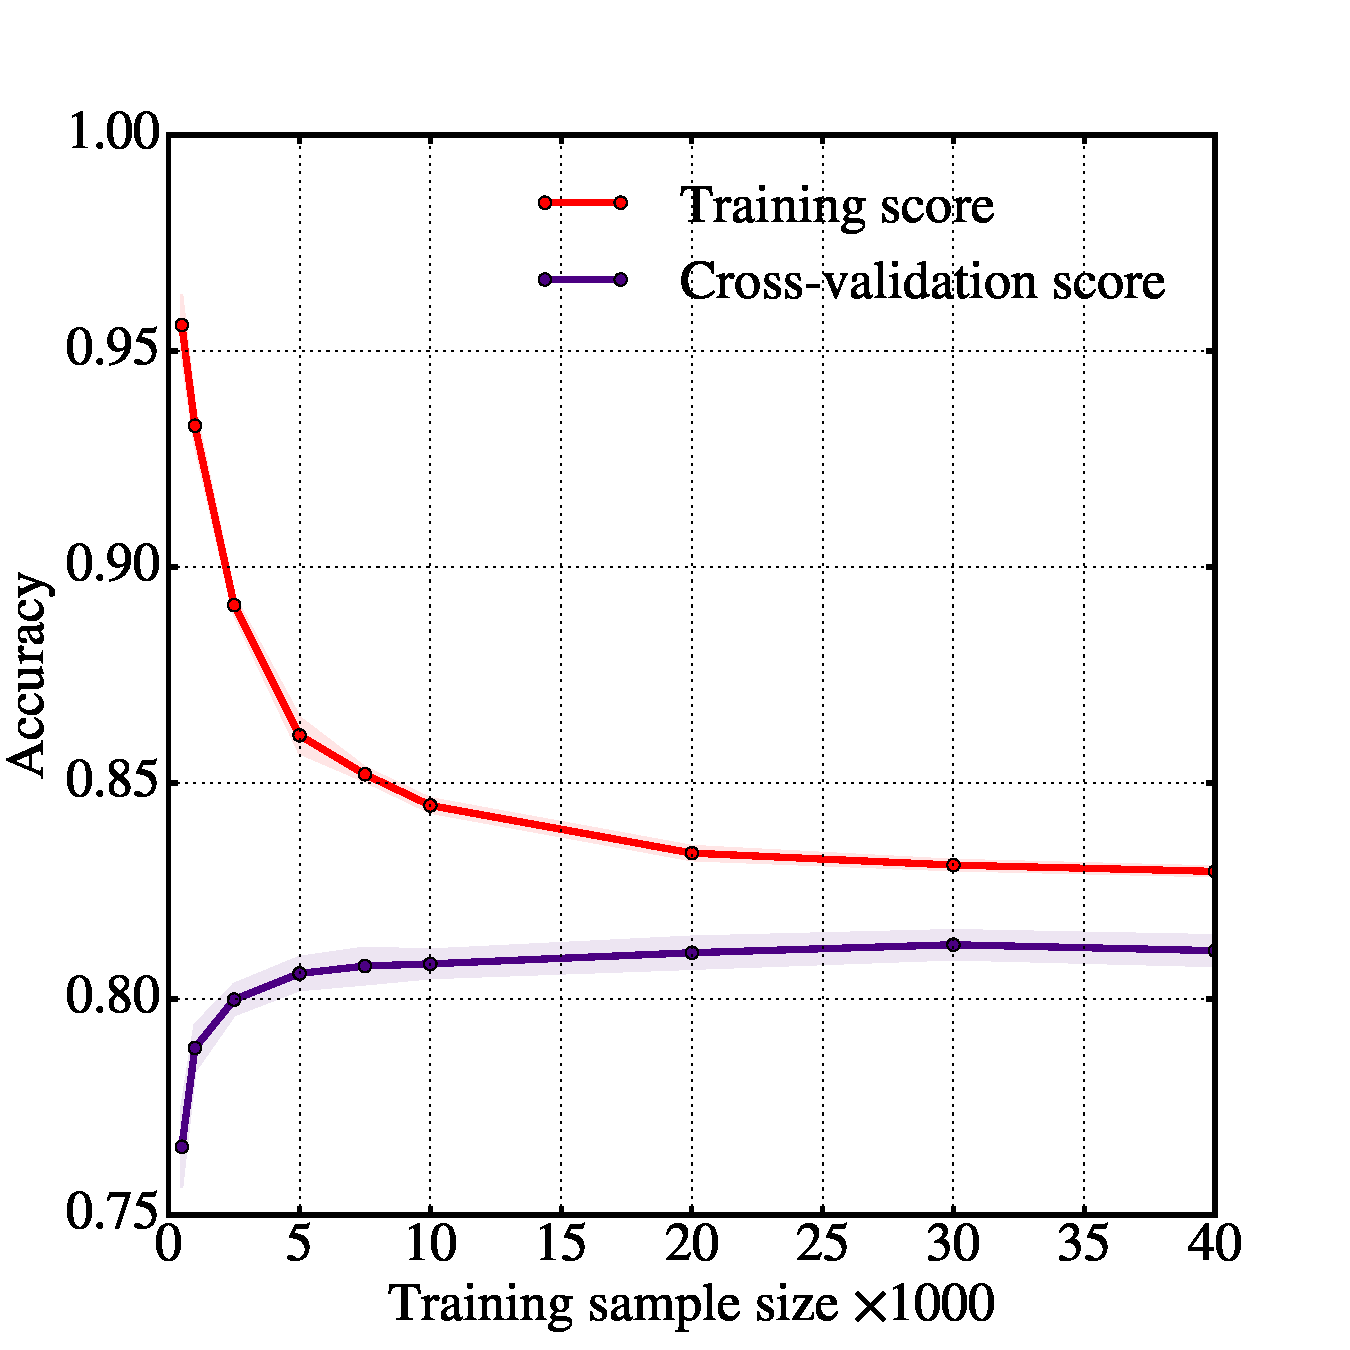
\includegraphics[width=3.25in]{figures/learning_curve_RF.pdf}
\caption{Learning curve for a Random Forest with fixed hyperparameters. The training score is the accuracy of the trained machine applied to its own training sample. The cross-validation score is the accuracy of the machine computed during the cross-validation process. When the training sample size is small, the machine accurately identifies its own training sample but is unable to generalize to unseen data as evidenced by a low cross-validation score. As the training sample size increases, the cross-validation score increases. This behavior plateaus indicating that larger training samples provide little in additional performance. \label{fig: learning curve}}
\end{figure}


%%----------------------------------------------------------------------------------------------------------------------------------------------------
%%   DECISION ENGINE 
%%----------------------------------------------------------------------------------------------------------------------------------------------------
\subsection{Decision Engine}\label{sec: decision engine}
A number of decisions must be addressed before attempting to train the machine. 
In particular, which subjects should be designated as the training sample? 
When should the machine attempt its first training session? 
When has the machine's performance been optimized such that it will successfully
generalize to unseen subjects? The field of machine learning provides few hard rules 
for answering these questions, only guidelines and best practices. 
Here we briefly discuss our approach for the development of our decision engine.


As discussed in detail in Section~\ref{sec: SWAP}, SWAP yields a probability that 
a subject exhibits the feature of interest. While some machine algorithms can 
accept continuous input labels, the RF requires distinct classes. We thus use only 
those subjects which have crossed either of the retirement thresholds. 
Though we find that SWAP consistently retires 35-40\%~\feat~subjects on 
any given day of the simulaton, a balanced ratio of~\feat~to~\notfeat~isn't guaranteed.
 Highly unbalanced training samples should be resampled to correct the imbalance; 
however, as we exhibit only a mild lopsidedness, we allow the machine to train on all 
SWAP-retired subjects.  

SWAP retires a few hundred subjects during the first days of the simulation.
In principle,  a machine can be trained with such a small sample, but will be unable
to generalize to unseen data. We estimate a minimum number of training samples
and the machine's ability to generalize by considering a learning curve, an illustration
of a machine's performance with increasing sample size for fixed hyperparameters. 
Figure~\ref{fig: learning curve} demonstrates such a curve wherein we plot
the accuracy from both the 10-fold cross-validation, and the trained machine
applied to its own training sample for a random sample of GZ2 subjects
required to be balanced between~\feat~and~\notfeat.  
We fix the RF's hyperparameters as follows: \texttt{max\_depth} $=8$, 
\texttt{n\_estimators } $=30$, and \texttt{max\_features} $=2$. 
When the sample size is small, the cross-validation score is low and the training 
score is high, a clear sign of over-fitting.  However, as the training 
sample size increases, the cross-validation score increases and eventually plateaus,
 indicating that larger training sets will yield little additional gain. 

We estimate this plateau begins when the training 
sample reaches 10,000 subjects and require SWAP retire at least this many 
 before the machine attempts its first training.  We estimate the machine 
has trained sufficiently if the cross-validation score fluctuates by less than 1\% 
for three consecutive nights of training to ensure we have reached the plateau.  
This requires that we record the machine's training performance each night, 
including how well it scores on the training sample, the 
cross-validation score, and the best hyperparameters. 

%%%-------------------------------------------------------
%%%  FIGURE:    FULL GZX PERFORMANCE
%%%-------------------------------------------------------
\begin{figure*}[t!]
\centering
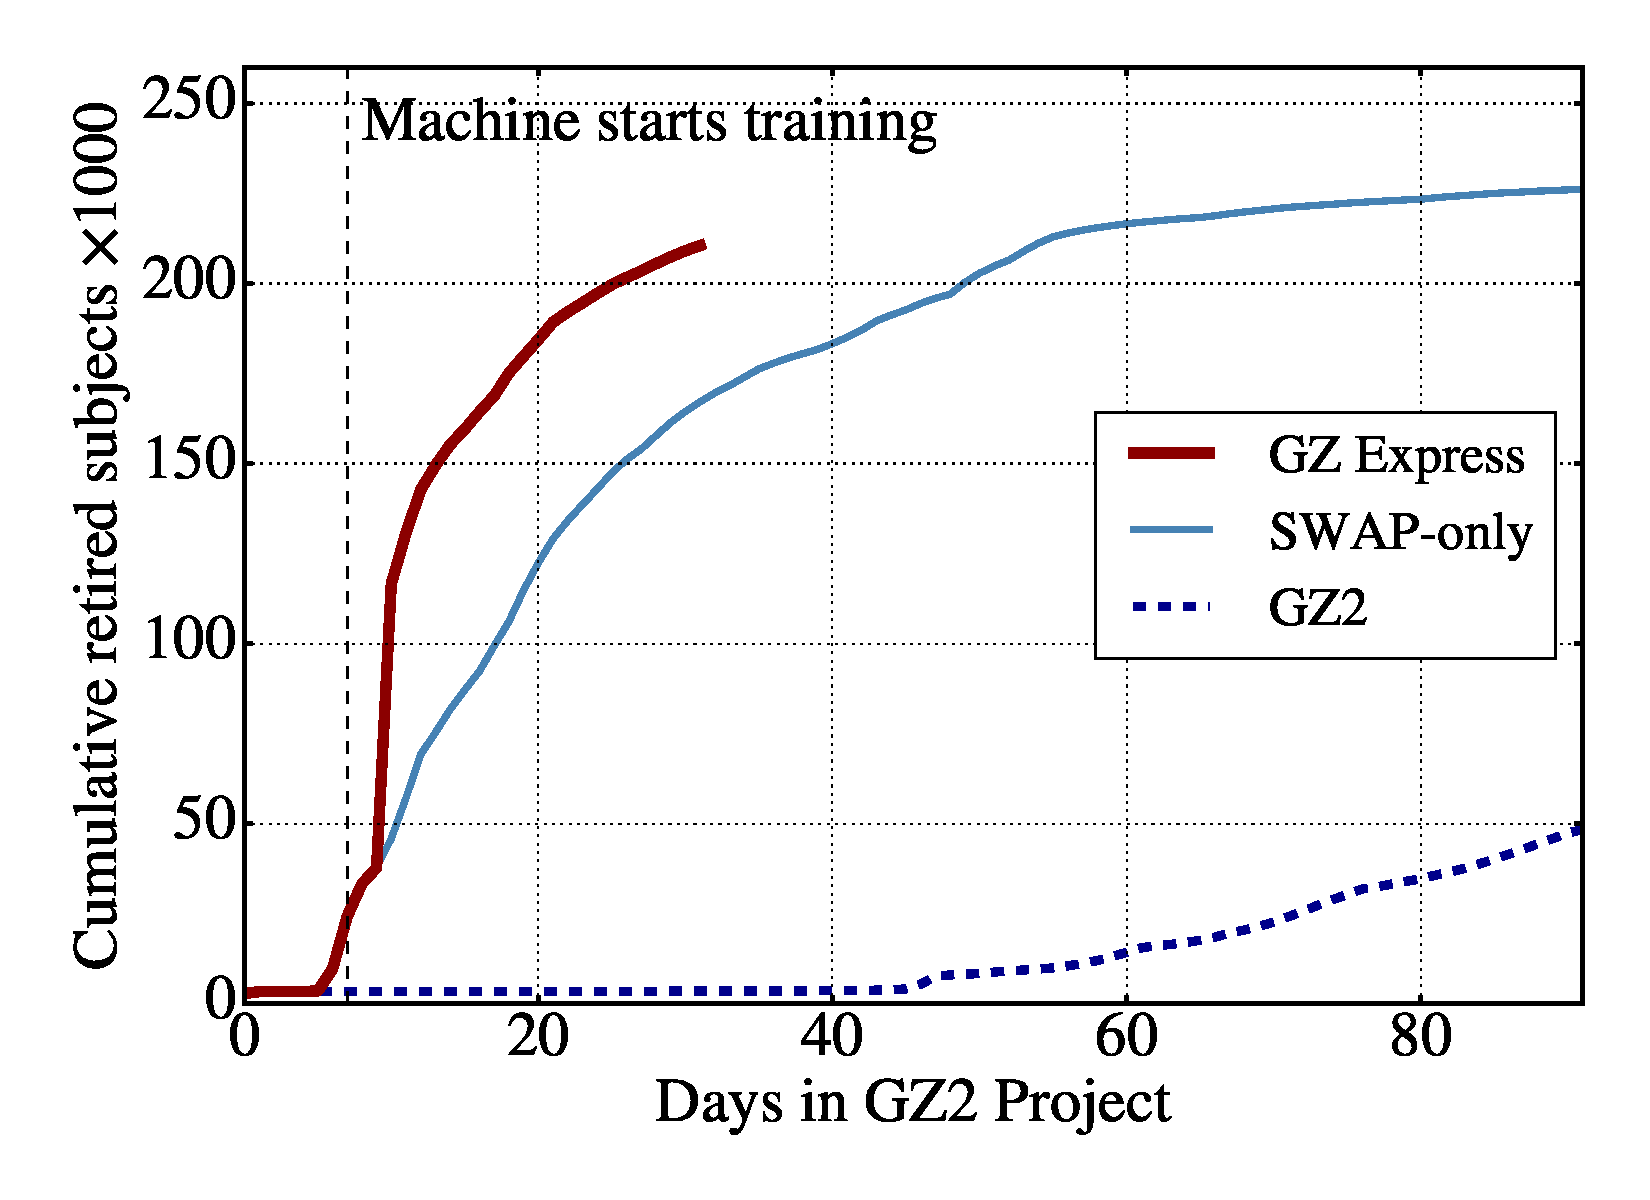
\includegraphics[width=5.5in]{figures/GZX_moneyplot.pdf}
\caption{By incorporating a machine classifier, GZX (red) increases the classification rate by an order of magnitude compared to GZ2 (dashed dark blue) and out-performs the SWAP-only run (light blue), retiring more than 200K subjects in just 27 days of GZ2 project time. The dashed black line marks the first night the machine trains. After several additional nights of training, it is deemed optimized and allowed to retire subjects. Both humans and machine then contribute to retirement. We end the simulation after 32 days having retired over 210K galaxies. See Table~\ref{tab: summary} for details. \label{fig: money}}
\end{figure*}


%%----------------------------------------------------------------------------------------------------------------------------------------------------
%%   MACHINE SHOP 
%%----------------------------------------------------------------------------------------------------------------------------------------------------
\subsection{The Machine Shop}\label{sec: machine shop}
We can now describe a full GZX simulation, which begins with human classifications 
processed through SWAP for several days.   
Once at least 10K subjects have been retired, their feature vectors are passed to 
the machine for its inaugural training. 
A suite of performance metrics are recorded by a machine agent, similar
in construction to SWAP's agents. This agent determines 
when the machine has trained sufficiently by assessing the variation
in performance metrics for all previous nights of training. 
Once the machine has been optimized, the agent introduces it to the test sample
consisting of any subject that has not yet reached retirement through SWAP 
and is not part of the gold standard sample.  

Analogous to SWAP, we generate a retirement rule for machine-classified subjects. 
In addition to the class prediction, the RF algorithm computes the probability for
each subject to belong to each class.  This probability is simply the average of
 the probabilities of each individual decision tree, where the probability of a 
single tree is determined as the fraction of subjects of class X on a leaf node.  
Only subjects that receive a class prediction with $p_{\mathrm{machine}} \ge 0.9$ are considered
retired. The remaining subjects have the possibility of being classified by humans 
or the machine on a future night of the simulation. 
This constitutes the core of our passive feedback mechanism. Subjects that are
not retired by the machine can instead be retired by humans, thus providing 
the machine a more fully sampled morphology parameter space on future 
training sessions. 



%%----------------------------------------------------------------------------------------------------------------------------------------------
%%   RESULTS 
%%----------------------------------------------------------------------------------------------------------------------------------------------
\section{Results} \label{sec: results}
We perform a full GZX simulation incorporating our RF with the fiducial 
SWAP run discussed in Section~\ref{sec: fiducial}. 
The machine attempts its first training on Day 8 with an initial training
sample of $\sim$20K subjects. It undergoes several additional nights 
of training, each time with a larger training sample. 
By Day 12, SWAP has provided over 40K subjects for training and the machine's 
agent has deemed the machine optimized. 
The machine predicts class labels for the remaining 230K GZ2 subjects. 
Of those, the machine retires over 70K, dramatically increasing the 
subset of retired subjects. 
We end the simulation after 32 days, having retired $\sim$210K subjects
as detailed in Table~\ref{tab: summary}. 

We present these results in Figure~\ref{fig: money} where subject retirement 
with GZX (red) is compared to our fiducial SWAP-only run (light blue) and GZ2 (dashed dark blue). 
Using the~\raw~labels as before, we compute our usual quality metrics on the 
full sample of GZX-retired subjects; reported in Table~\ref{tab: summary}. 
Accuracy and purity remain within a few percent of the SWAP-only run at 93.5\% 
and 84.2\% respectively. Instead we see a 5\% decline in the completeness. 
While the SWAP-only run identified 99\% of~\feat~subjects, incorporation
of the machine seems to miss a significant portion thus dropping GZX completeness to 94.3\%. 
We discuss this behavior below.

By dynamically generating a training sample through a more sophisticated analysis of 
human classifications coupled with a machine classifier, we retire more than 200K 
GZ2 subjects in just 27 days.  Visual classification through SWAP alone retires as 
many in 50 days, while GZ2 requires a full year.  
GZX thus provides an order of magnitude increase in the rate of classification
over the traditional crowd-sourced approach. 
We next explore the composition of those classifications.

\begin{table*}[]
	\centering
	\caption{Summary of key quantities for GZ2 and our various simulations. All quality metrics are calculated using~\raw~labels.}
	\label{tab: summary}
	\let\mc\multicolumn
	\begin{tabular}{lcccccc}
		
		\mc7c{ \textbf{Simulation Summary} } \\
		\hline \hline
			& Days	& Subjects Retired & Human Effort 	&  Accuracy 	& Purity 	& Completeness\\
		\mc2c{} 		& 	 	& (classifications) 	&  (\%)	    	& (\%)	& (\%)	\\
		\hline
			
		Galaxy Zoo 2	&	430 	& 285962  	& 16,340,298 	& --   	& --    	 & --   \\
		SWAP only	&	92    	& 226124          & 2,298,772	& 95.7 	& 86.7	 & 99.0     \\
		SWAP+RF   	& 32  	& 210543 	& 932,017 	& 93.5    	& 84.2    	& 94.3      \\
		\hline
	\end{tabular}
\end{table*}

%%----------------------------------------------------------------------------------------------------------------------------------------------
%%   WHO RETIRES WHAT, WHEN? 
%%----------------------------------------------------------------------------------------------------------------------------------------------
\subsection{Who retires what, when?}  

In the top panel of Figure~\ref{fig: gzx components} we explore the individual 
contributions to GZX subject retirement from the RF (dash-dotted yellow) and SWAP (dashed red). 
The solid black line shows the total GZX retirement (SWAP+RF), while the dotted grey line depicts 
the fiducial SWAP-only run from Section~\ref{sec: fiducial} for reference. 
Two things are immediately obvious. First, each component shoulders approximately
half of the retirement burden with the machine and SWAP responsible for $\sim$$100$K and $\sim$$110$K subjects respectively.  
	Secondly, the rate of retirement exhibited by the two components is in stark contrast.
SWAP retires at a relatively constant rate while the machine retires 
dramatically at the beginning of its application, quickly surpassing the human 
contribution, and plateaus thereafter. 


%%%-------------------------------------------------------
%%%  FIGURE:    GZX COMPONENT CONTRIBUTIONS
%%%-------------------------------------------------------
\begin{figure}[t!]
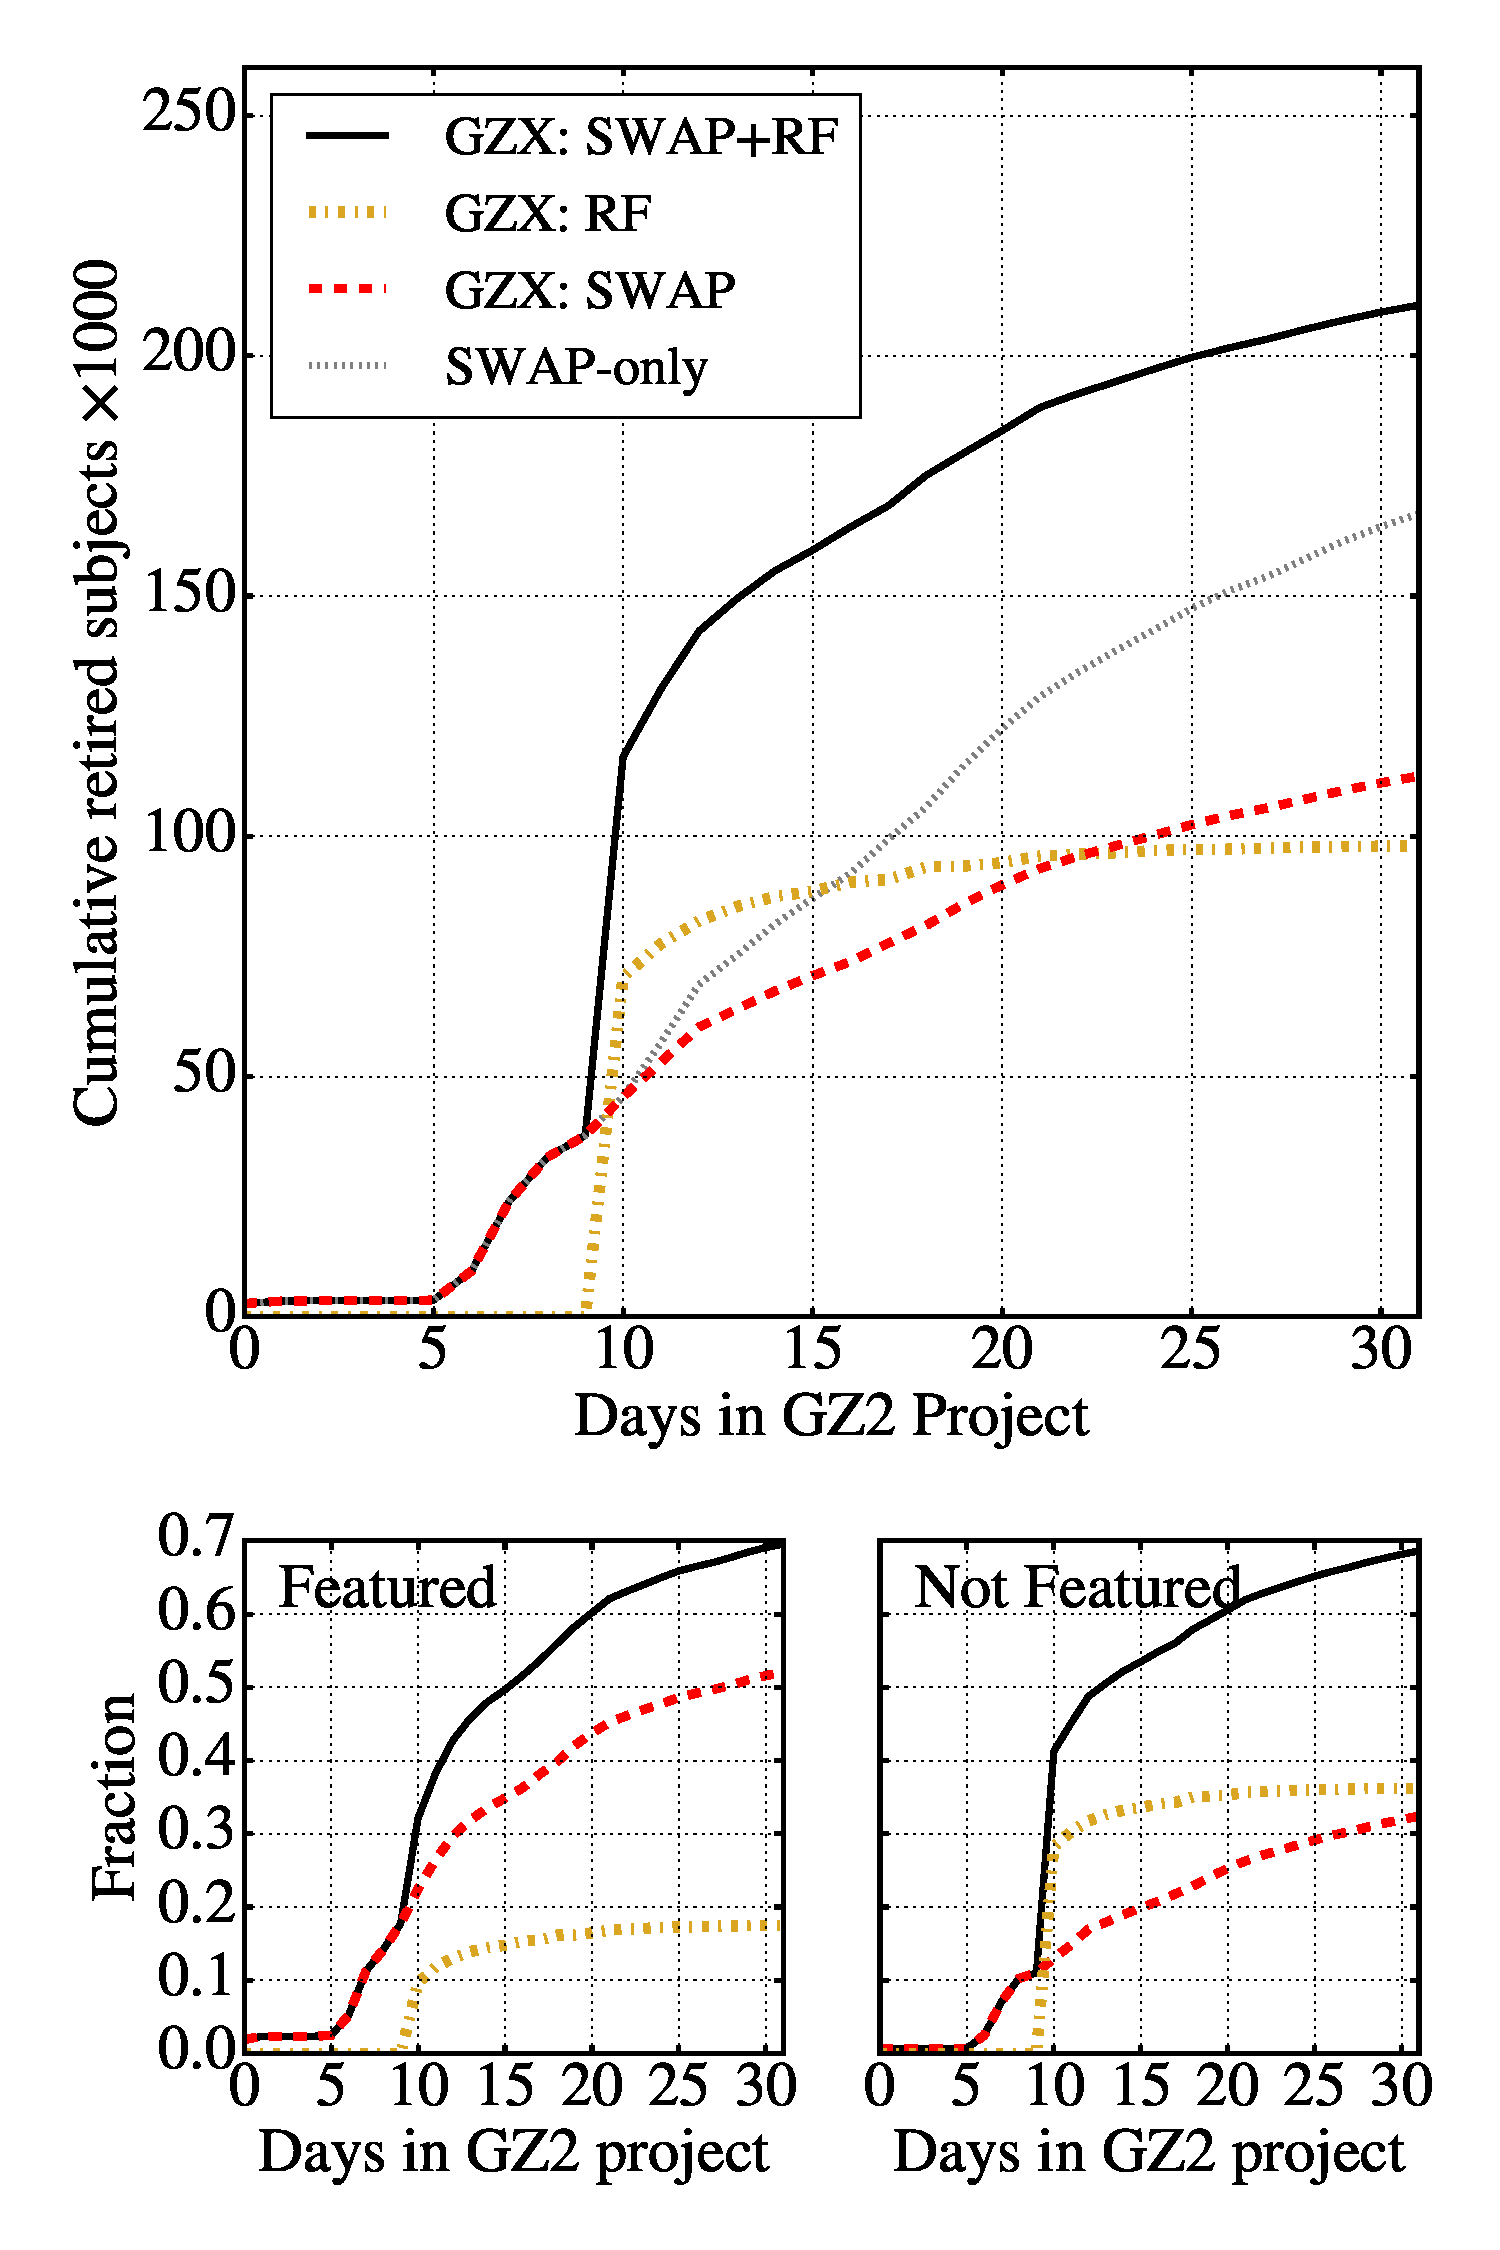
\includegraphics[width=3.5in]{figures/GZX_component_contributions.pdf}
\caption{Contributions to subject retirement by both classifying agents of GZX: human (SWAP) and machine. The top panel shows cumulative subject retirement for GZX as a whole (solid black), along with that attributed to the RF (dash-dotted yellow), and SWAP (dashed red). The dotted grey line shows the fiducial SWAP-only run for comparison. Retirement totals for humans and machine are nearly equal over the course of the simulation but display different behaviors: SWAP's retirement rate is almost constant while the RF contributes substantially after its initial application and then plateaus.  The bottom panels show what fraction of GZ2 subjects are retired, separated by class label. Overall, GZX retires 73.6\% of the entire GZ2 sample in 32 days, retiring the same proportion of~\feat~and~\notfeat~subjects as indicated by the black lines. However, humans retire 30\% more~\feat~subjects than the machine, while both components retire a similar proportion of~\notfeat~subjects. \label{fig: gzx components}}
\end{figure}

%%%-------------------------------------------------------
%%%  FIGURE:    MACHINE GETS IT RIGHT!!!
%%%-------------------------------------------------------
\begin{figure*}[t!]
\centering
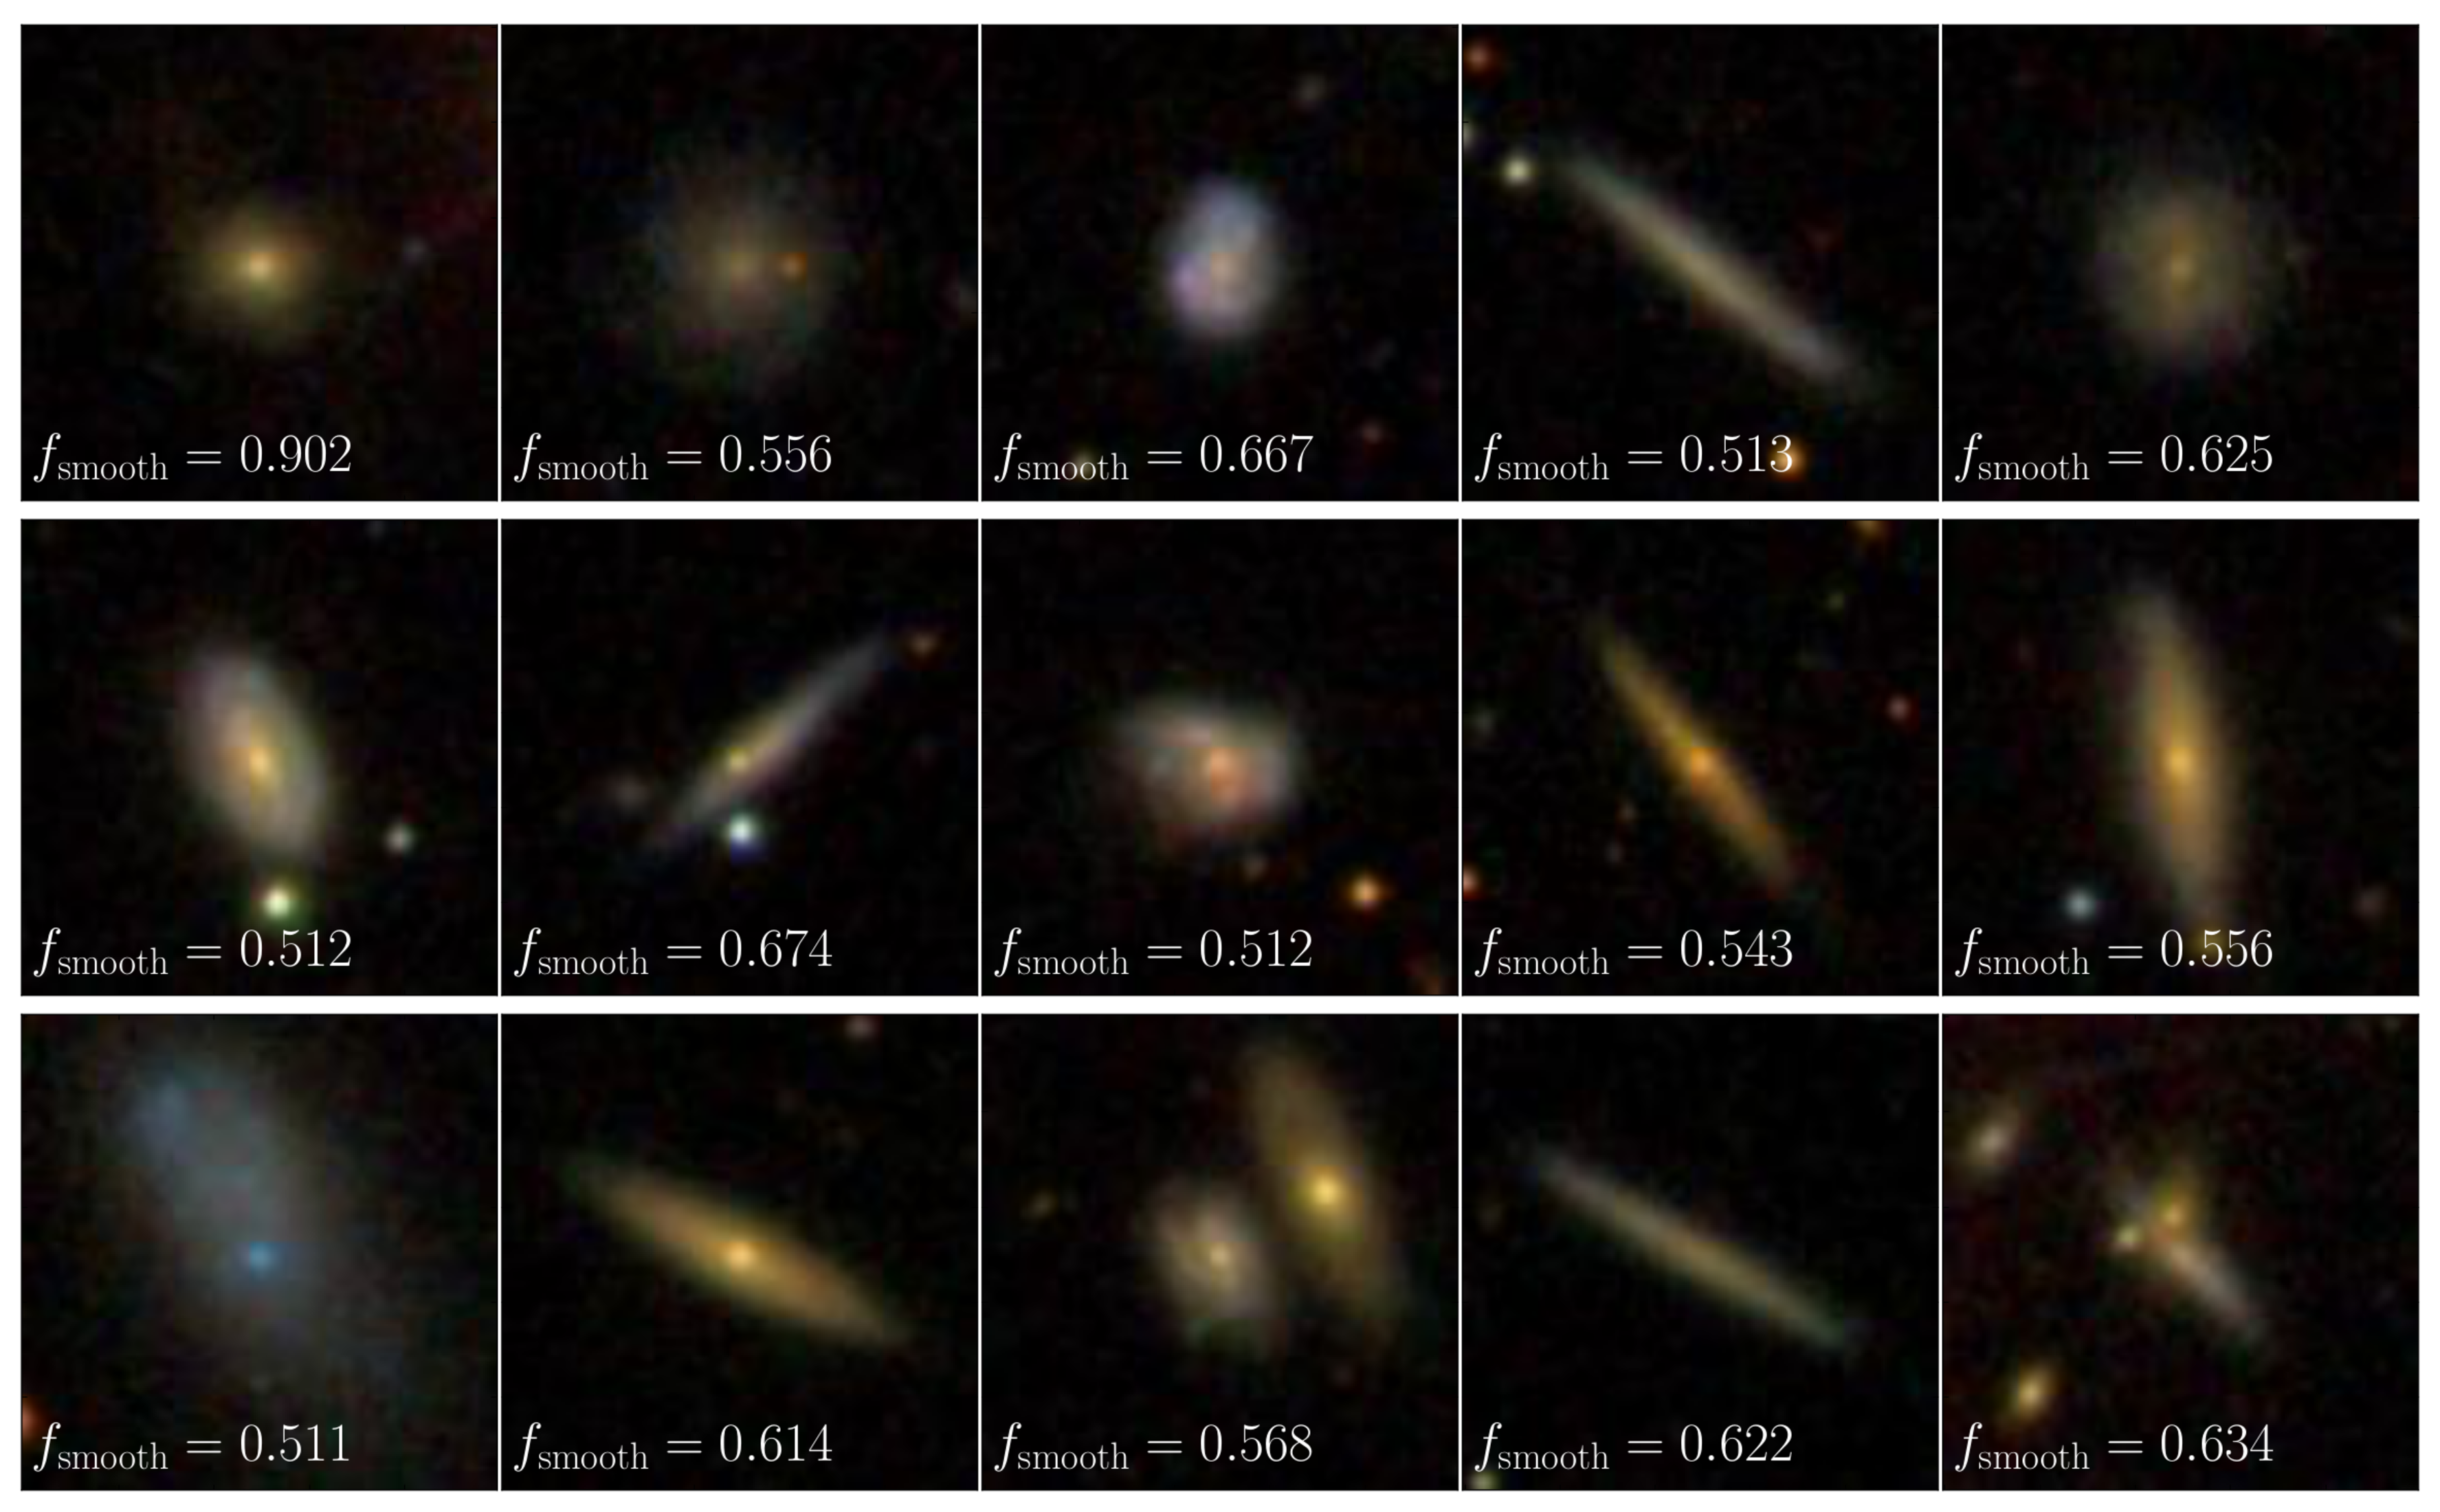
\includegraphics[width=6.5in]{figures/machine_false_positives_jpgs.pdf}
\caption{A random subsample of subjects identified as false positives: labeled by machine as~\feat, but as~\notfeat~according to~\raw. We display \fsmooth~in the lower left corner, that is, the fraction of volunteers who classified the subject as `smooth' (\notfeat). Values are typically between 0.5 and 0.65 indicating that GZ2 volunteers did not reach a strong consensus. Fortunately, the machine is able to identify these subjects as~\feat~due to their measured morphology diagnostics. \label{fig: machine false pos}}
\end{figure*}

We thus clearly see three epochs of subject retirement, as we presumed.
In the first phase, humans are the only contributors to subject retirement.  
Once the machine is optimized, it immediately contributes more to retirement than humans.
However, the machine's performance plateaus quickly;  the third 
phase is again dominated by human classifications.

In the bottom panels of Figure~\ref{fig: gzx components}, we consider the class
composition of subjects retired by SWAP and the RF. 
The left (right) panel shows the retired fraction of GZ2 subjects identified 
as~\feat~(\notfeat) according to their~\raw~labels as a function of GZ2 project time. 
Overall, GZX retires 73.6\% of the GZ2 subject sample and this is evenly 
distributed between~\feat~and~\notfeat~subjects as indicated by the solid
black lines in both panels. 
However, SWAP retires more than 50\% of all~\feat~subjects while the machine
retires only 18\%. This divergence does not exist for~\notfeat~subjects where
each component contributes 33-37\%. 

What is the source of this discrepancy? 
Each night the machine trains on a sample composed consistently of 30-40\%~\feat~subjects but does not retire a similar proportion, indicating
that the 30\% of non-retired~\feat~subjects do not receive high~\pmachine. 
In the following section we explore whether this is an artifact of our choice in machine 
or in the human-machine combination implemented here. 


\subsection{Machine performance}\label{sec: machine performance}

Throughout our analysis we have defined~\feat~and~\notfeat~subjects by 
their~\raw~labels as this was the most compatible choice for comparison with SWAP output.  
However, the machine does not learn in the same way, nor is it presented with the 
same information. We argue that the machine classifications are valid 
and complimentary to human classifications. 

Of the 6127 subjects that were deemed false positives, i.e., galaxies retired by the 
machine as~\feat~that have~\notfeat~\raw~labels, we visually examine several hundred
and assess that, to the expert eye, a majority are, in fact, \feat.  
A random sample is shown in Figure~\ref{fig: machine false pos}, where the value 
in the lower left corner is the raw GZ2 smooth vote fraction, \fsmooth; 
the fraction of volunteers who classified that subject as~\notfeat. 
This small sample consists predominantly of edge-on disks and disk 
galaxies with low surface brightness features. 

That the machine can identify~\feat~galaxies that humans classify 
as~\notfeat~has two contributing factors: 
1) the first task of the GZ2 decision tree asks a very specific question that 
does not necessarily correlate with a split between early- and late-type galaxies, and 
 2) the machine learns on morphology diagnostics that are very different from visual inspection. 
Regarding the first point, the full sample of false positives has $\langle f_{\mathrm{smooth}} \rangle = 0.645 \pm 0.106$  with 56.7\%  having \fsmooth~$\le 0.65$. This indicates that volunteers have not 
reached a strong consensus for a majority of these subjects; behavior that could 
be modified by providing actual training images and live feedback as performed in \cite{Marshall2016}. 
We note that 71.7\% of these galaxies are labeled~\feat~after GZ2's debiasing process. 

%%%-------------------------------------------------------
%%%  FIGURE:   CAS DISTRIBUTIONS 
%%%-------------------------------------------------------
\begin{figure*}[t!]
\centering
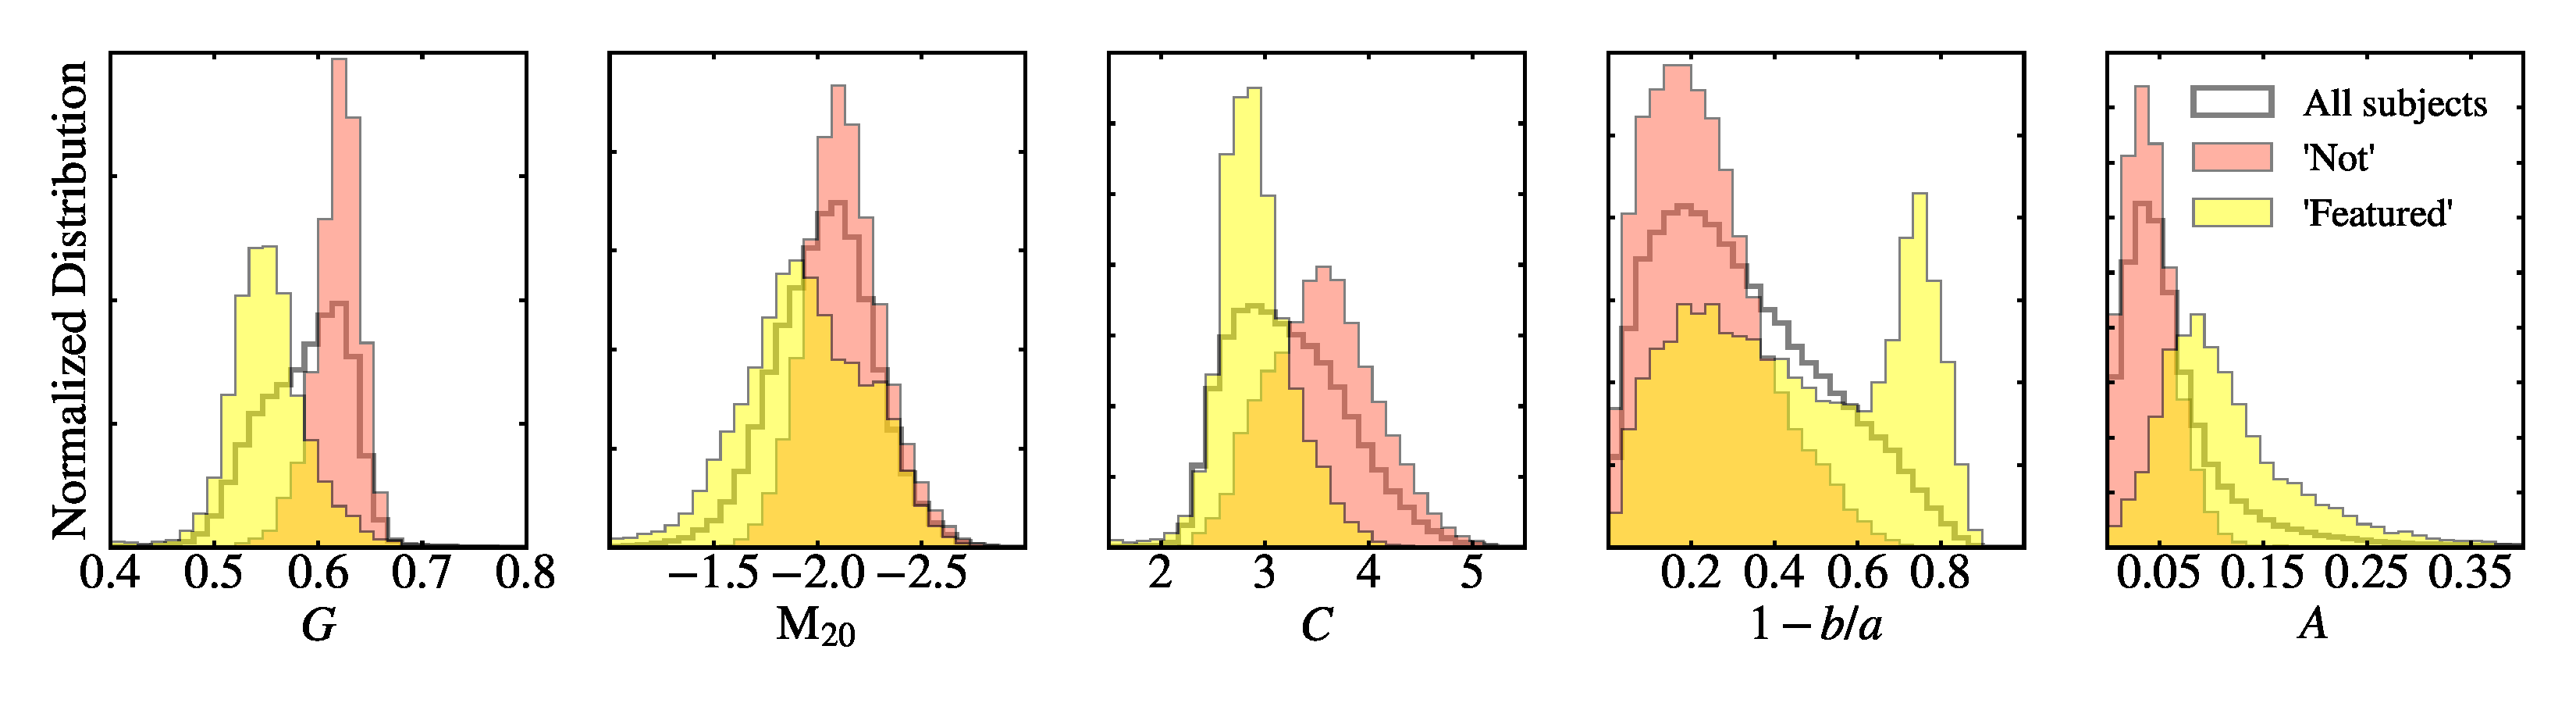
\includegraphics[width=7in]{figures/machine-retired_morph_params.pdf}
\caption{The RF is trained on a 5-dimensional morphology parameter space. We show the distribution of each morphology indicator for machine-retired~\feat~(yellow) and~\notfeat~(not yellow) subjects compared to the full GZ2 subject sample (black). The difference between~\feat~and~\notfeat~subjects is in stark contrast for all distributions except, perhaps, \M{20}.  \label{fig: morph params}}
\end{figure*}


%%%-------------------------------------------------------
%%%  FIGURE:   FEATURE IMPORTANCES
%%%-------------------------------------------------------
\begin{figure}[t]
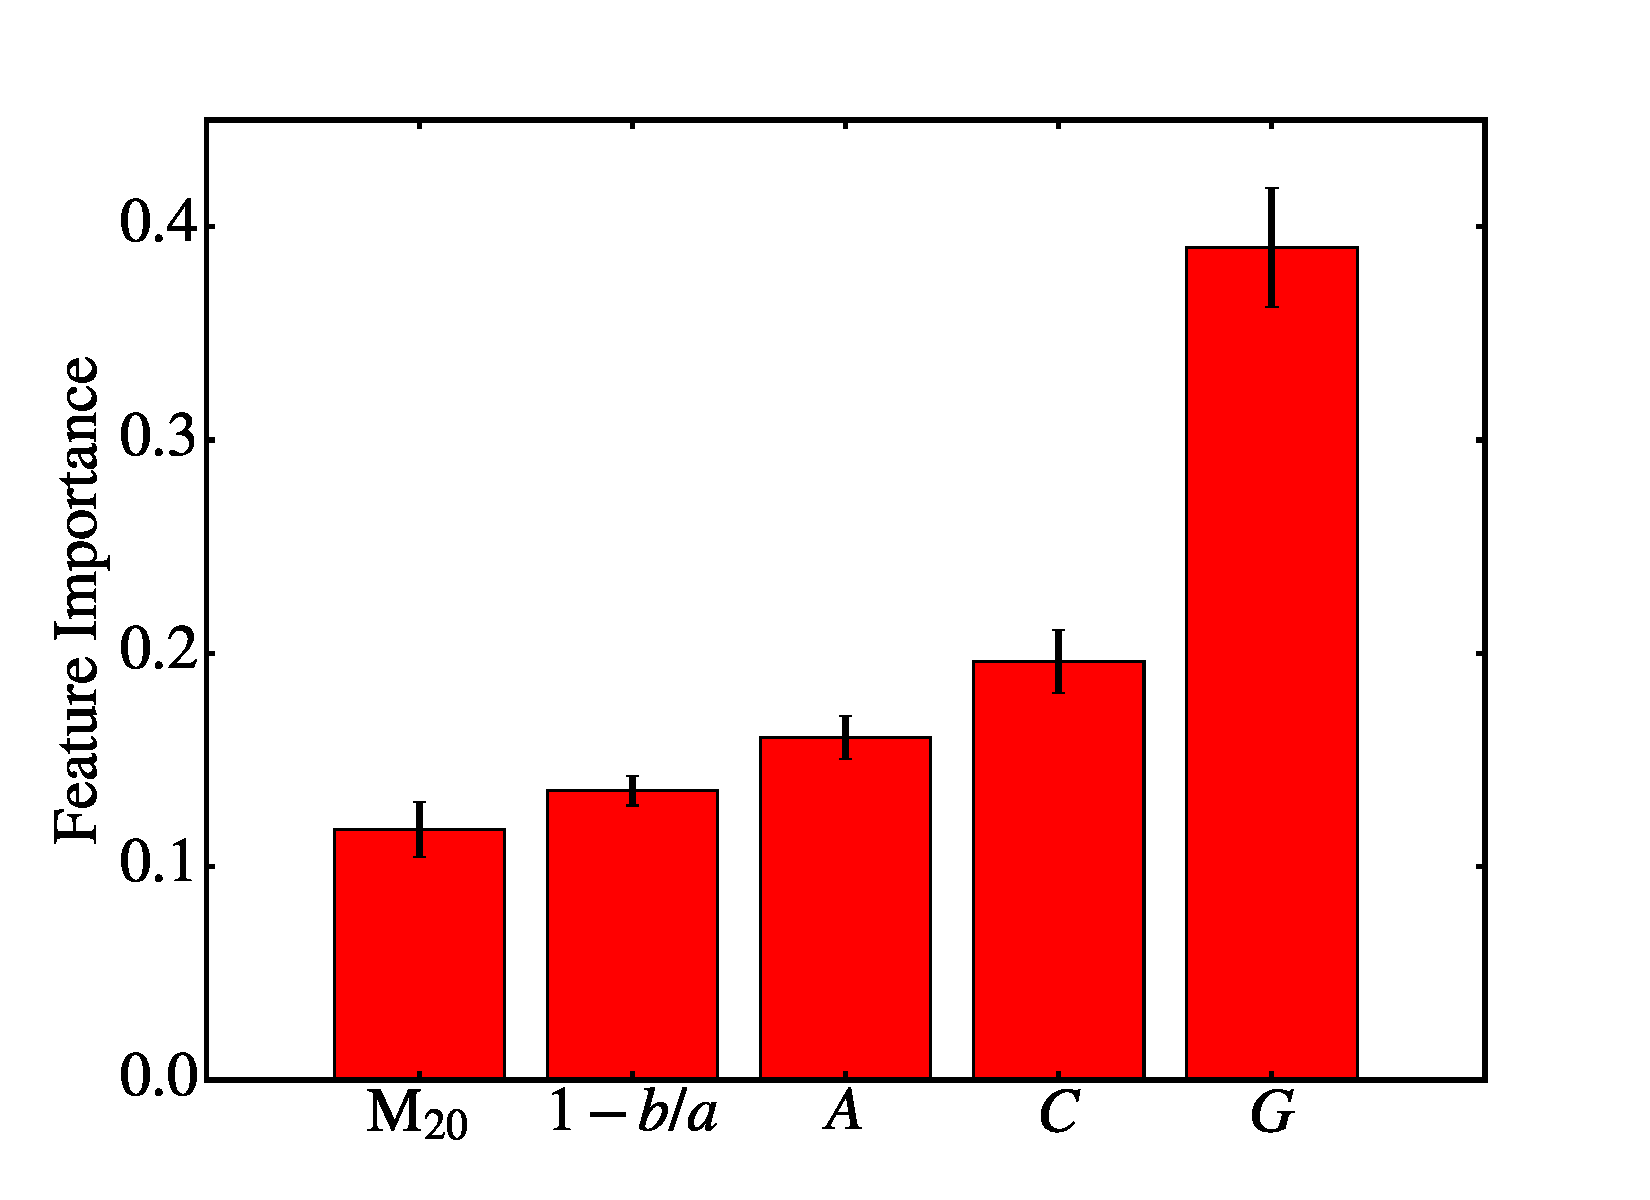
\includegraphics[width=3.5in]{figures/RF_feature_importances_4paper.pdf}
\caption{The RF's ranked feature importance averaged over all nights of training with black bars indicating the standard deviation. A larger value corresponds to higher importance. The machine computes feature importance according to how much each feature increases the purity of the resulting split averaged over all trees in the forest. The RF places great importance in the Gini coefficient though we note that it can under-represent the importance of highly correlated features such as concentration.\label{fig: feature importance}}
\end{figure}

The second point suggests that, in some cases, the morphology indicators we measure are 
sufficient for the machine to recognize~\feat~galaxies regardless of the labels humans provide. 
Figure~\ref{fig: morph params} shows the distribution of each 
morphology indicator for all subjects the machine retires as~\feat~(yellow) 
and~\notfeat~(not yellow) compared to the full GZ2 subject set. 
The difference between~\feat~and~\notfeat~is stark in all but the \M{20} distribution. 
This can be seen explicitly in Figure~\ref{fig:  feature importance} where
we show the RF's ranked feature importances with large values indicating higher importance. 
Feature importance is computed as how much each feature decreases the impurity 
of a split in a tree. The impurity decrease from each feature is then averaged over
all trees and ranked. 
We show the feature importance averaged over all nights of training with 
black bars indicating the standard deviation. The machine finds the Gini coefficient 
most important for class prediction, and places little emphasis on \M{20}. 
It is well known that the Gini coefficient is more sensitive to noise than other diagnostics, 
however, we point out that when a machine is faced with two or more correlated features, 
any of them can be used as the predictor. Once chosen, the importance of the others is reduced. 
This explains why Concentration is ranked much lower than Gini even though they 
are strongly correlated as seen in Figure~\ref{fig: morph thresh}. 
That the machine relies heavily on these two morphology diagnostics is unsurprising as
concentration has long been an automated predictor between early- and late-type galaxies~\citep{Abraham1994, Abraham1996, Shen2003}.


The complementary nature of human and machine classification can 
best be utilized by a feedback mechanism in which a portion of machine-retired
subjects are reviewed by humans. Subjects that display excessive disagreement
should be verified by an expert (or expert-user).  In the same way that 
humans increase the machine's training sample over time, subjects that the
machine properly identifies can become part of the humans' training sample. 



%%----------------------------------------------------------------------------------------------------------------------------------------------------
%%   MAD RAVINGS OF THE FUTURE 
%%----------------------------------------------------------------------------------------------------------------------------------------------------
\section{Looking Forward}\label{sec: visions}

We have demonstrated the first practical framework for combining human and machine
 intelligence in galaxy morphology classification tasks. 
While we focus below on a brief discussion of our next steps and potential applications
to large upcoming surveys, we note that our results have implications for the future
of citizen science and Galaxy Zoo in particular. 


GZX is perhaps one of the simplest ways to combine human and machine intelligence
 and its impressive performance motivates a higher level of sophistication. 
A first step will be an implementation of SWAP that can handle a complex decision tree. 
In addition, we envision multiple forms of active feedback in addition to 
our passive feedback mechanism.  SWAP allows us to leverage the 
most skilled volunteers to review galaxies difficult for either
 human or machine to classify.  Additionally, machine-retired subjects should 
contribute to the training sample for humans in an analogous fashion to what 
we have already implemented. 


Secondly, our RF can be improved by providing it information equal to what
humans receive: multi-band morphology diagnostics will be
included in our future feature vector.  However, the Random Forest algorithm is not 
easily adapted to handle measurement errors or class labels with continuous distributions. 
To fully utilize the information provided by SWAP, sophisticated algorithms such as 
deep convolutional neural networks (CNN) or Latent Dirichlet allocation (LDA), 
an algorithm that is frequently used in document processing, should be considered.  
Furthermore, there is no reason to limit to a single machine. 
As hinted at in Figure~\ref{fig: schematic}, several machines could train simultaneously, 
their predictions aggregated through SWAP, creating an on-the-fly machine ensemble.

%%----------------------------------------------------------------------------------------------------------------------------------------------------
%%  IMPLICATIONS FOR UPCOMING LARGE-SCALE SURVEYS
%%----------------------------------------------------------------------------------------------------------------------------------------------------

With the above upgrades implemented, we expect performance of both the
classification rate and quality to further increase. However, even our current 
implementation can cope with upcoming data volumes from large surveys. 
By some estimates, \textit{Euclid} is expected to obtain measurable morphology with its 
visual instrument (VIS) for approximately $10^6 - 10^7$ galaxies~\citep{Euclid}.
Visual classification at the rate achieved with Galaxy Zoo today
would require 12--120 years to classify.\footnote{We note that the classification 
rate of GZ2 was 4 times higher than GZ's current steady rate.}
If the \textit{Euclid} sample is on the high end, GZX as currently implemented
could classify the brightest 20\% during the six years of its observing mission. 
As currently implemented, we obtain accuracy around 95\% potentially leaving
hundreds of thousands of galaxies with unreliable classifications.  
In a companion paper that seeks to identify supernovae, Wright et al. (submitted) 
demonstrate a dramatic increase in accuracy through an entirely different human-machine 
combination whereby the
scores from human and machine are averaged together with the combined score 
yielding the most reliable classification. Again, a combination of both 
approaches will allow us to take full advantage of legacy output from large scale surveys.


%%----------------------------------------------------------------------------------------------------------------------------------------------------
%%   CONCLUSIONS 
%%----------------------------------------------------------------------------------------------------------------------------------------------------
\subsection{Conclusions}

In this paper we design and test Galaxy Zoo Express, an innovative system\footnote{Our code can be found at \url{https://github.com/melaniebeck/GZExpress}} 
for the efficient classification of galaxy morphology tasks that integrates the 
native ability of the human mind to identify the abstract and novel with 
machine learning algorithms that provide speed and brute force.  
We demonstrate for the first time that the 
SWAP algorithm, originally developed to identify rare gravitational lenses in the 
Space Warps project, is robust for use in galaxy morphology classification. 
We show that by implementing
SWAP on GZ2 classification data we can increase the rate of classification by a factor
of 4-5, requiring only 90 days of GZ2 project time to classify nearly 80\% of the
entire galaxy sample. 

Furthermore, we have implemented and tested a Random Forest algorithm 
and developed a decision engine that delegates tasks between human and 
machine.  We show that even this simple machine is capable of providing significant 
gains in the classification rate when combined with human classifiers: GZX
 retires over 70\% of GZ2 galaxies in just 32 days of GZ2 project time.  
This represents a factor of 11.4 increase in the classification rate as well as
 an order of magnitude reduction in human effort compared to the original GZ2 project. 
This is achieved without sacrificing the quality of classifications as we maintain 
accuracy well above 90\% throughout our simulations. 
Additionally, we have shown that training on a 5-dimensional parameter space of 
traditional non-parametric morphology indicators allows the machine to identify 
subjects that humans miss, providing  a complementary approach to visual classification. 
The gain in classification speed allows us to tackle the massive amounts of data soon
to be forthcoming from large surveys like \textit{LSST} and \textit{Euclid}.


%%----------------------------------------------------------------------------------------------------------------------------------------------------
%%   ACKNOWLEDGEMENTS
%%----------------------------------------------------------------------------------------------------------------------------------------------------
\acknowledgements
MB thanks Steven Bamford and Boris H{\"a}u{\ss}ler for insightful discussions on citizen science and Galaxy Zoo; and John Wallin and Marc Huertas-Company for several enlightening conversations on machine learning and classification. 
We are grateful to Elisabeth Baeten, Micaela Bagley, Karlen Shahinyan, Vihang Mehta, Steven Bamford, Kevin Schawinski, and Rebecca Smethurst for providing expert classifications in addition to those provided by the authors. PJM acknowledges Aprajita Verma and Anupreeta More for their ongoing collaboration on the Space Warps project. 

MB, CS, LF, KW, and MG gratefully acknowledge support from the US National Science
Foundation Grant AST-1413610.  MB acknowledges additional support 
through New College and Oxford University's Balzan Fellowship as well as the University
of Minnesota Doctoral Dissertation Fellowship. Travel funding was supplied 
to MB, in part, by the University of Minnesota Thesis Research Travel Grant. CJL recognizes support from a grant from the Science \& Technology Facilities Council (ST/N003179/1). 
BDS acknowledges support from Balliol College, Oxford, and the National Aeronautics and Space Administration (NASA) through Einstein Postdoctoral Fellowship Award Number PF5-160143 issued by the Chandra X-ray Observatory Center, which is operated by the Smithsonian Astrophysical Observatory for and on behalf of NASA under contract NAS8-03060. The work of PJM is supported by the U.S. Department of Energy under contract number DE-AC02-76SF00515.

\software{scikit-learn \citep{scikit-learn}, Astropy \citep{astropy}, TOPCAT \citep{topcat}}



%%----------------------------------------------------------------------------------------------------------------------------------------------------
%%   APPENDIX
%%----------------------------------------------------------------------------------------------------------------------------------------------------
\appendix
\label{sec:Appendix}


%% ----------------------------------------------------------------------------------------------------------------------------------------------
%% 		EXPLORING SWAP PARAMETERS
%% ----------------------------------------------------------------------------------------------------------------------------------------------
\section{Exploring SWAP's Parameter Space} \label{sec: tweaking swap}

In this Appendix we explore the SWAP parameter space and assess the effects on subject retirement. 


\textbf{Initial agent confusion matrix.} 
In our fiducial simulation each volunteer was assigned an agent whose confusion matrix was
initalized at $(0.5, 0.5)$, which presumes that volunteers are no better than random classifiers.  
We perform two simulations wherein we initilize agent confusion matrices as $(0.4, 0.4)$, 
slightly obtuse volunteers; and $(0.6, 0.6)$, slightly astute volunteers, with everything else remaining constant.  
Results of these simulations compared to the fiducial run are shown in the left panel of
Figure~\ref{fig: tweak swap}. We find that SWAP is largely insensitive to the 
initial confusion matrix  both in terms of the subject retirement rate and classification quality.  

%% -------------------------------------------------------------------------------
%%   FIGURE:  SWAP --  CONFUSION MATRIX & PRIOR 
%% -------------------------------------------------------------------------------
\begin{figure*}[t]
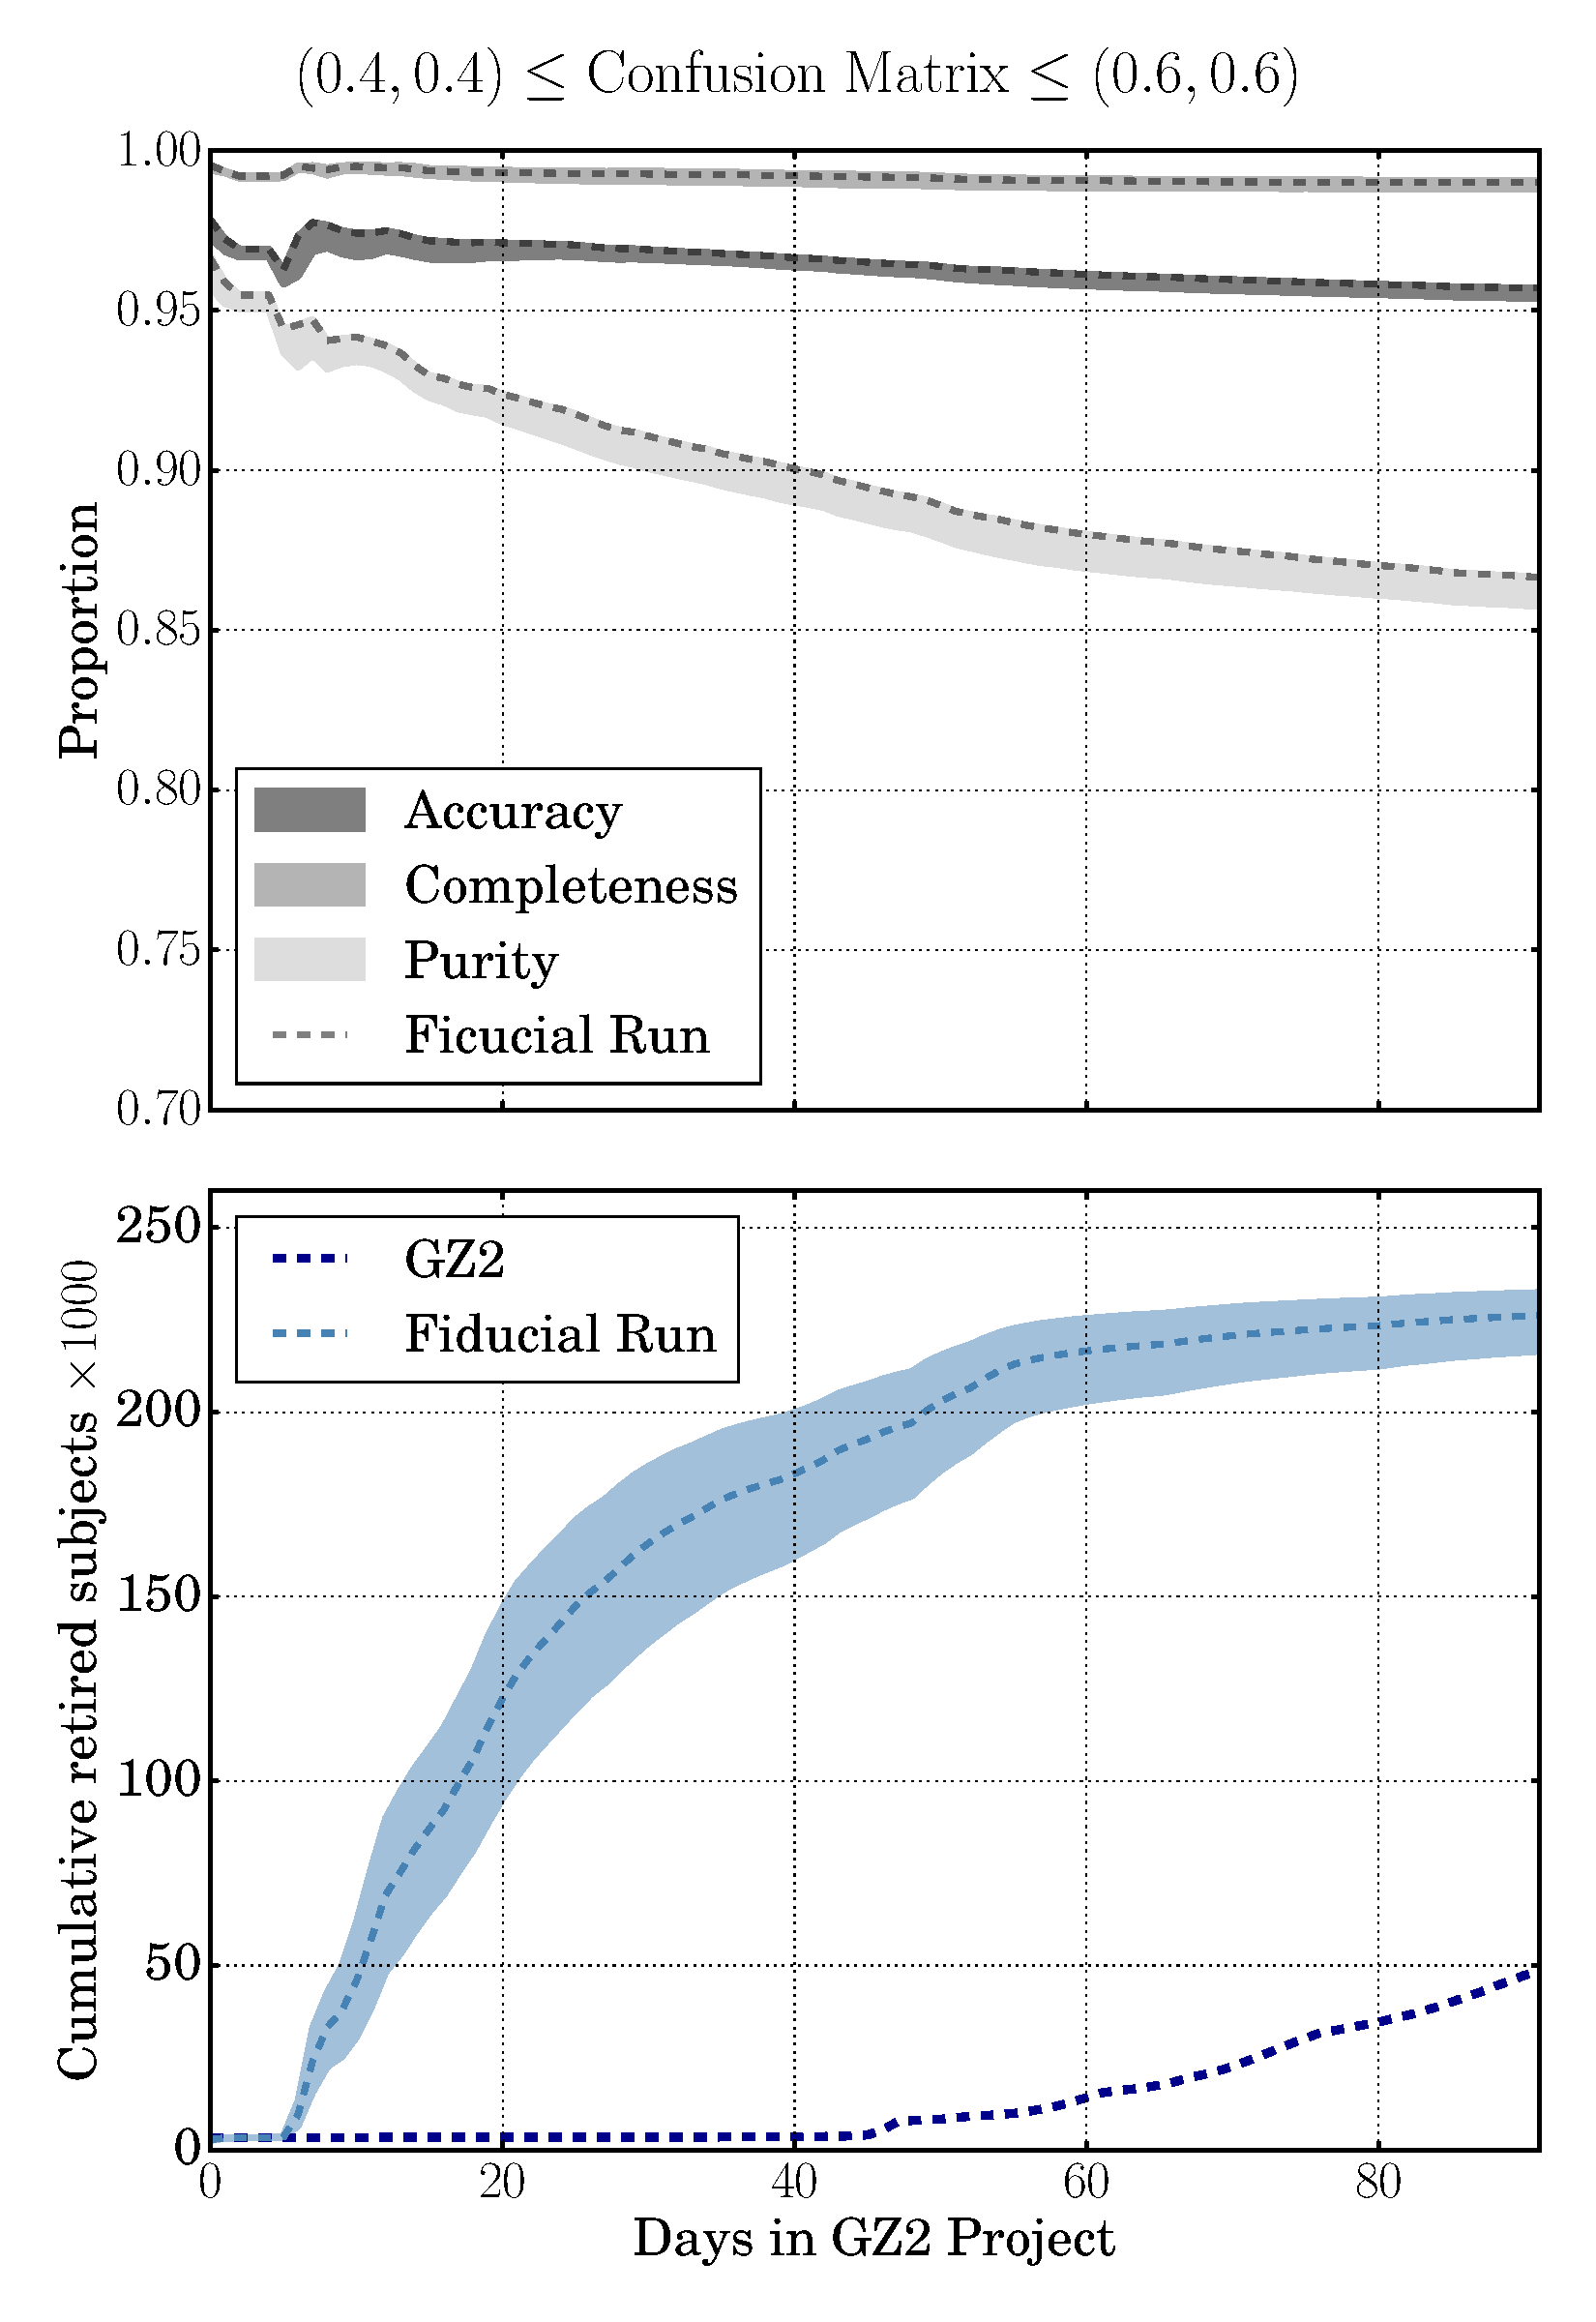
\includegraphics[width=3.35in]{figures/GZX_eval_and_retirement_PLPD_spread_4paper_v2.pdf}
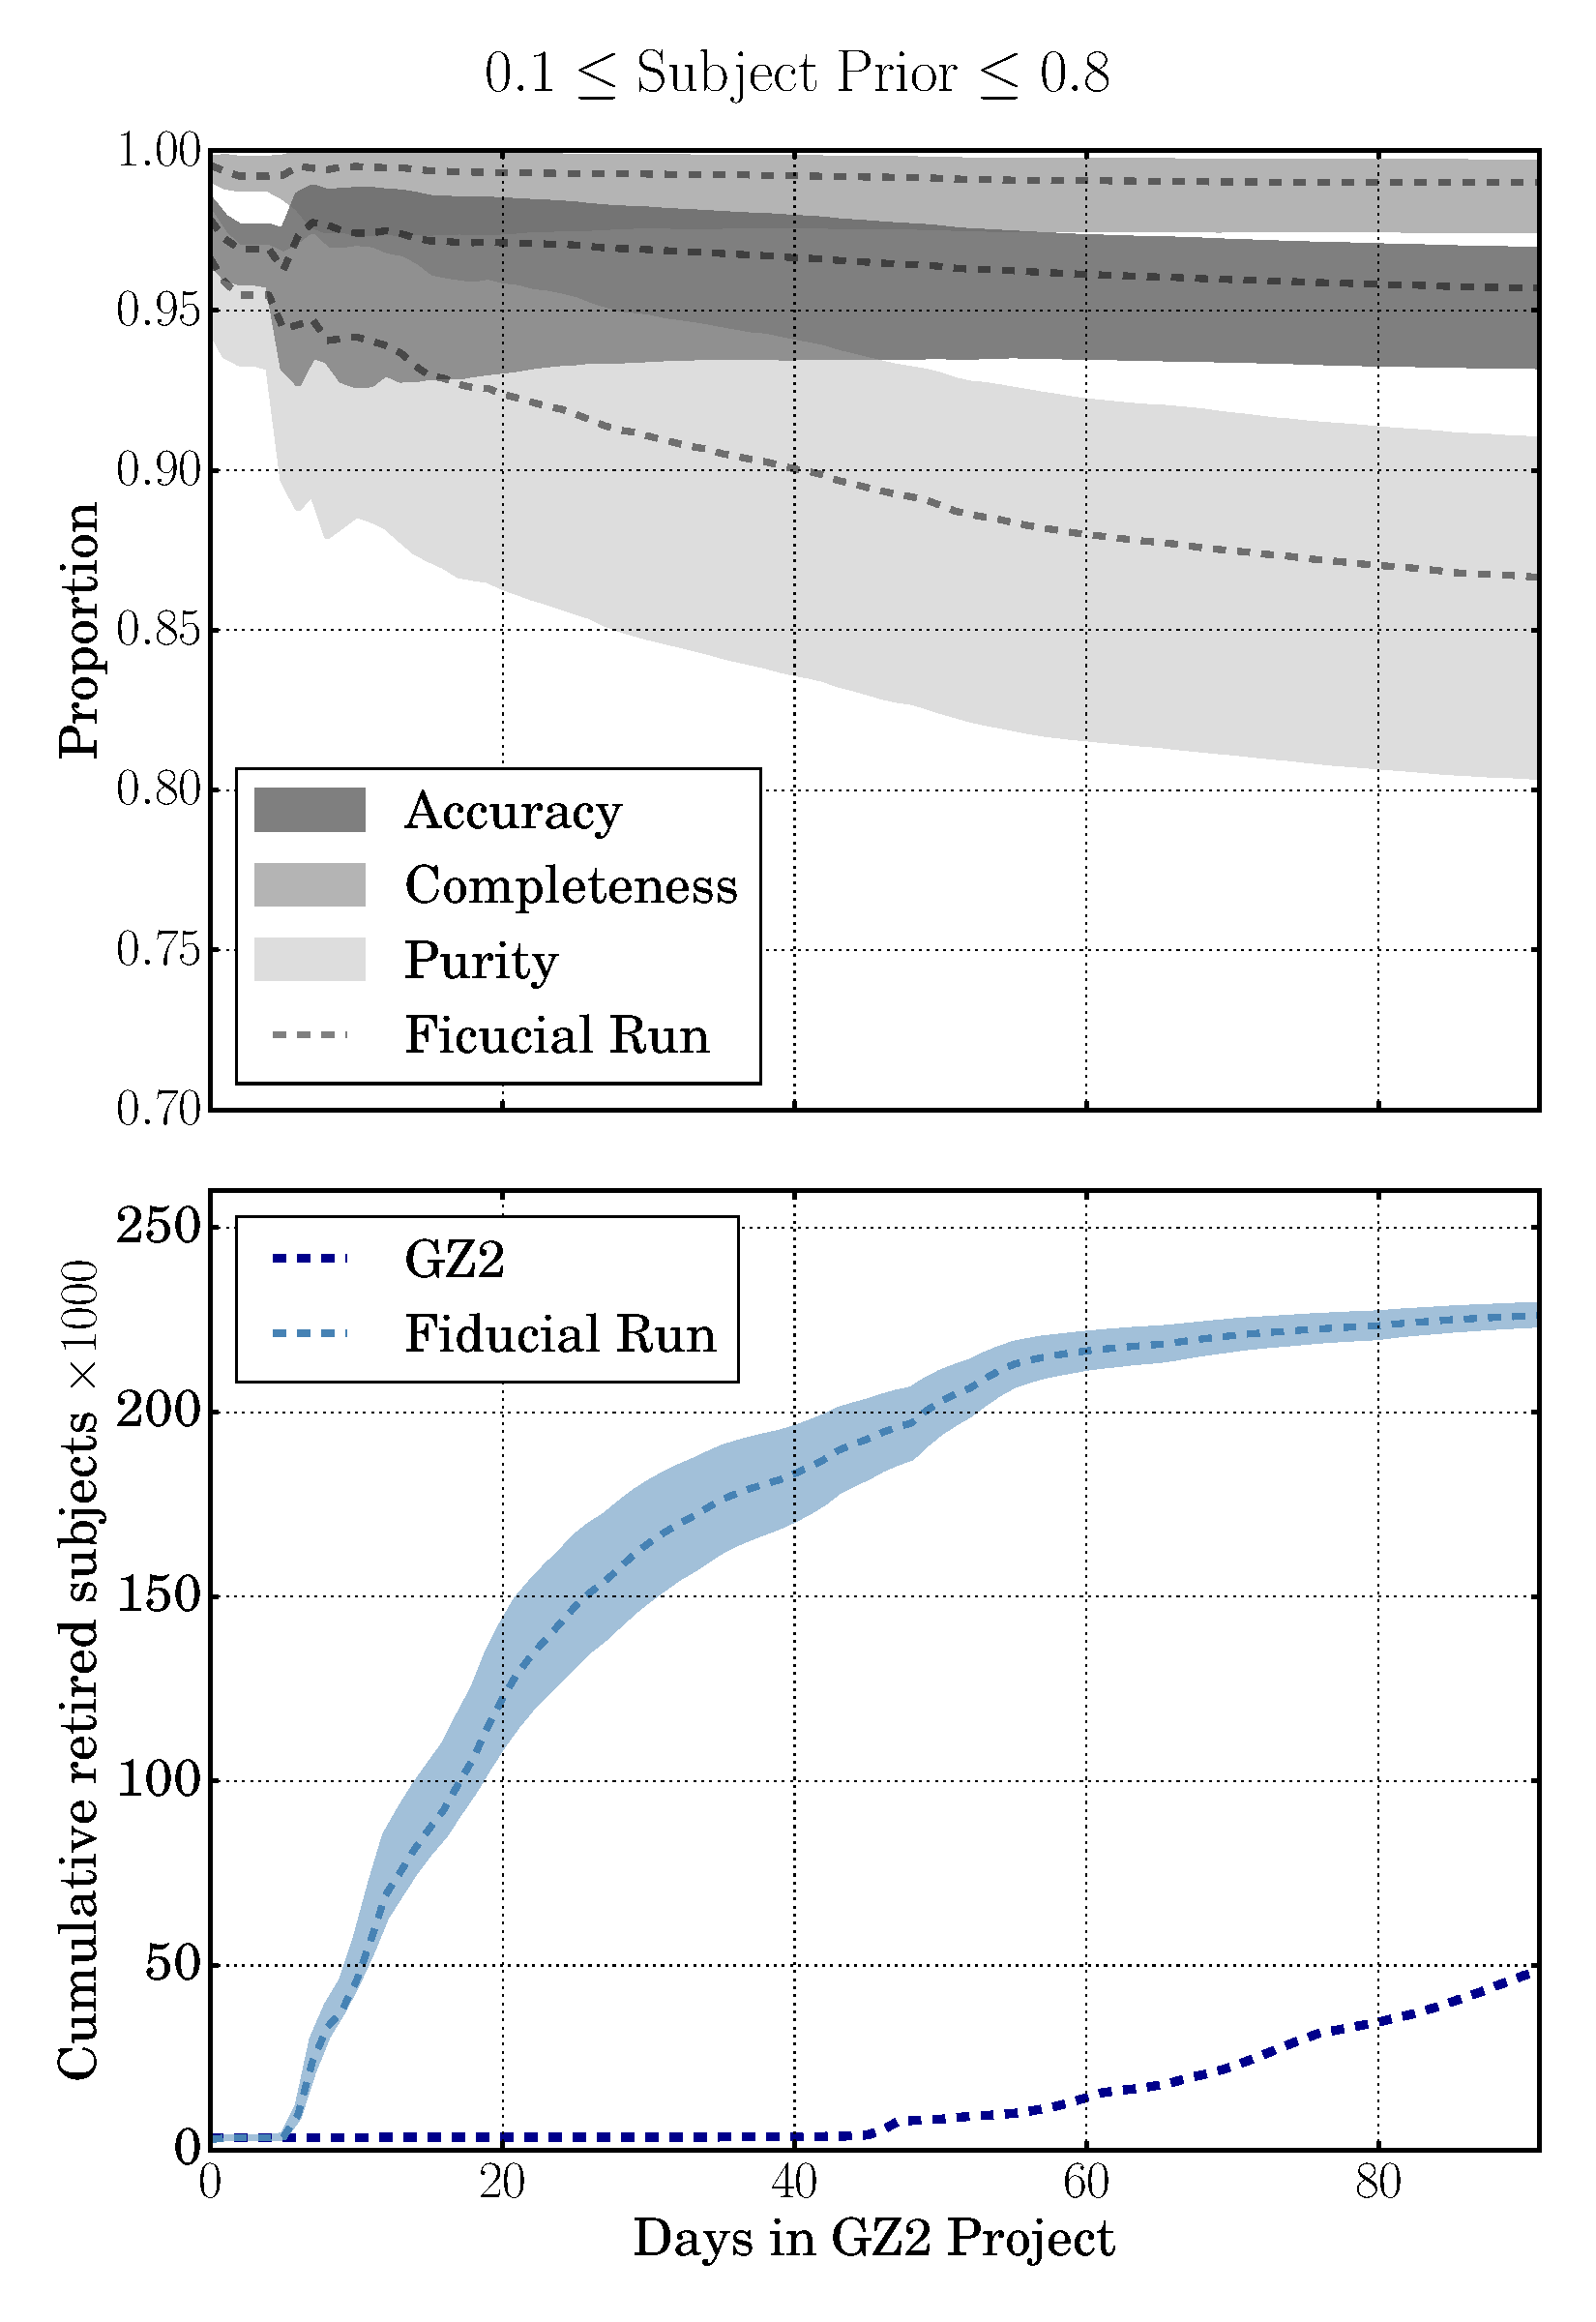
\includegraphics[width=3.35in]{figures/GZX_eval_and_retirement_prior_spread_4paper_v2.pdf}
\caption{SWAP performance does not dramatically change even with a range of input parameters as compared to the fiducial run of Section~\ref{sec: fiducial} (dashed lines).  \textit{Left.} The quality (top) and retirement rate (bottom) when the confusion matrix is initialized as (0.4, 0.4) and (0.6, 0.6), with all other input parameters remaining constant. \textit{Right.} Same as the left panel but allowing the subject prior probability, \p $= 0.2, 0.35$ and $0.8$. Changes in the confusion matrix have little impact on the quality of the labels but varies the total number of subjects retired. In contrast, changing the subject prior is more likely to affect the classification quality rather than the total number of subjects retired. \label{fig: tweak swap}}
\end{figure*}

We retire $\sim$$225$K$\pm3.5\%$ subjects as shown by the light blue shaded region in the bottom
left panel of Figure~\ref{fig: tweak swap}, where the dashed blue line denotes the fiducial run. 
Predictably, when the confusion matrix probabilities are low, we retire fewer subjects 
than when these probabilities are high for a given period of time. 
This is easy to understand since it takes longer for volunteers to become astute 
classifiers when they are initially given values denoting them as obtuse. 
Regardless, most volunteers become astute classifiers by the end of the simulation. 
The top left panel demonstrates our usual quality metrics as computed in Section \ref{sec: fiducial}.
The dashed lines again denote the fiducial run. 
We maintain $\sim$$95\%$ accuracy, $99\%$ completeness, and $\sim$$84\%$ purity;
 and no metric changes by $> 2\%$ regardless of initial confusion matrix values.  
 
This spread is due to three effects: 
1) subjects can receive an alternate SWAP label in different simulations, 
2) subjects can be retired in a different order, and 
3) the set of retired subjects is not guaranteed to be common to all runs. 
We find SWAP to be highly consistent: 
more than 99\% of retired subjects are the same among all simulations, 
and, of these, 99\% receive the same label.  Instead we find that the order in which 
subjects are retired changes between runs. 
When the confusion matrix is low, subjects take longer to classify compared to the fiducial run 
(i.e., they retire on a later date in GZ2 project time). 
Likewise, subjects retire sooner when the confusion matrix is high. 
This can cause quality metrics to vary since they are calculated on a day to day basis. 
These effects each contribute less than one per cent variation and thus we see a 
high level of consistency between simulations. 

Of interest, perhaps, is that the quality metrics for these simulations are not symmetric 
about the fiducial run. However, in the Bayesian framework of SWAP, an agent with 
confusion matrix (0.4, 0.4) contributes as much information as an agent with confusion matrix (0.6, 0.6).
The quality metrics computed are thus within a per cent of each other.
In either case, we find that initializing agents at (0.5, 0.5) provides optimal performance 
for the `training' we simulate with our current approach. Further assessment would 
require a live project with real-time training and feedback. 


%%%-------------------------------------------------------
%%%  FIGURE:   MORPH PARAMS & SWAP THRESHOLDS
%%%-------------------------------------------------------
\begin{figure*}[t!]
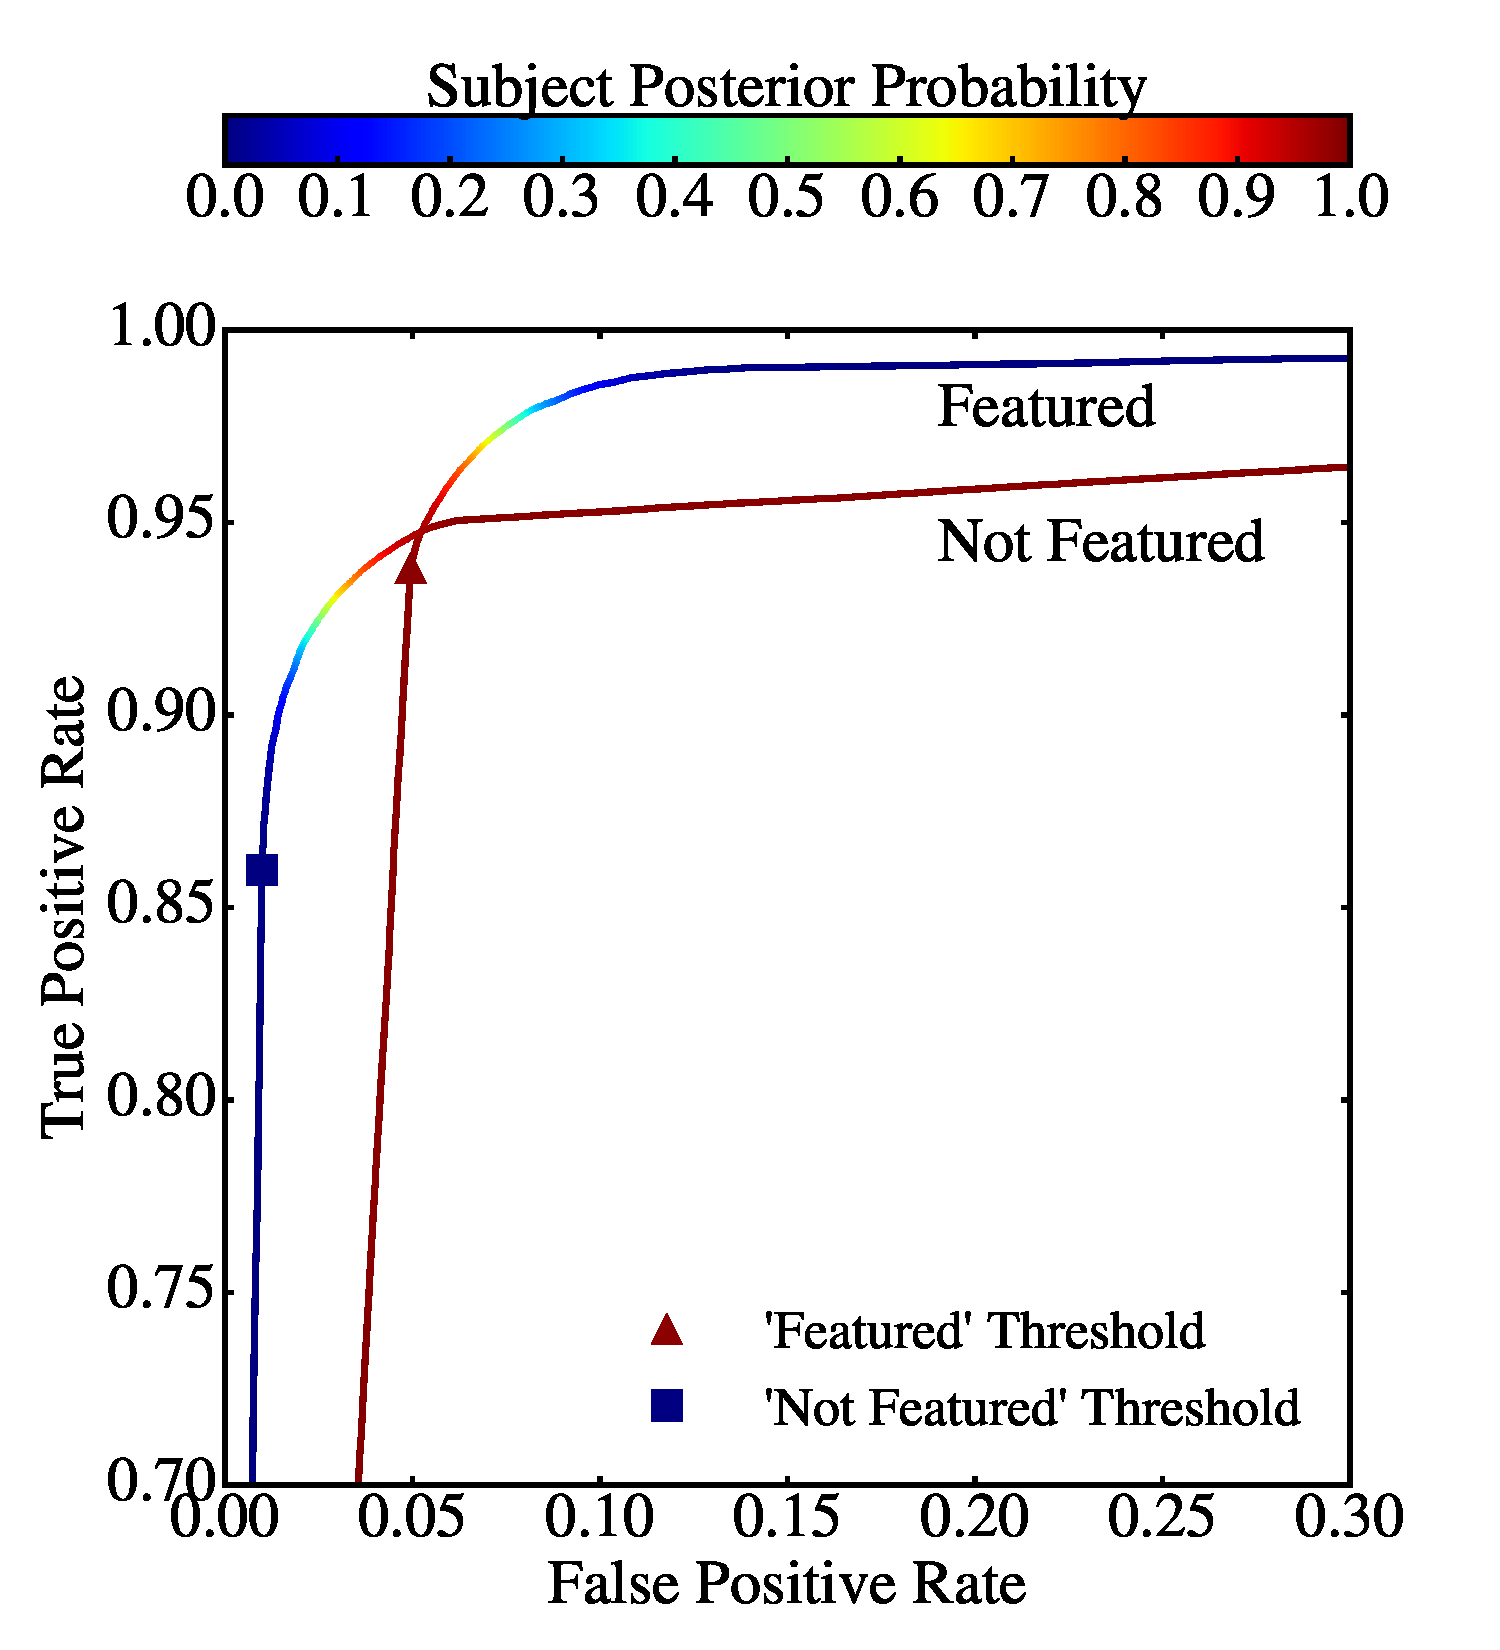
\includegraphics[width=3.08in]{figures/SWAP_ROC_curve_4paper.pdf}
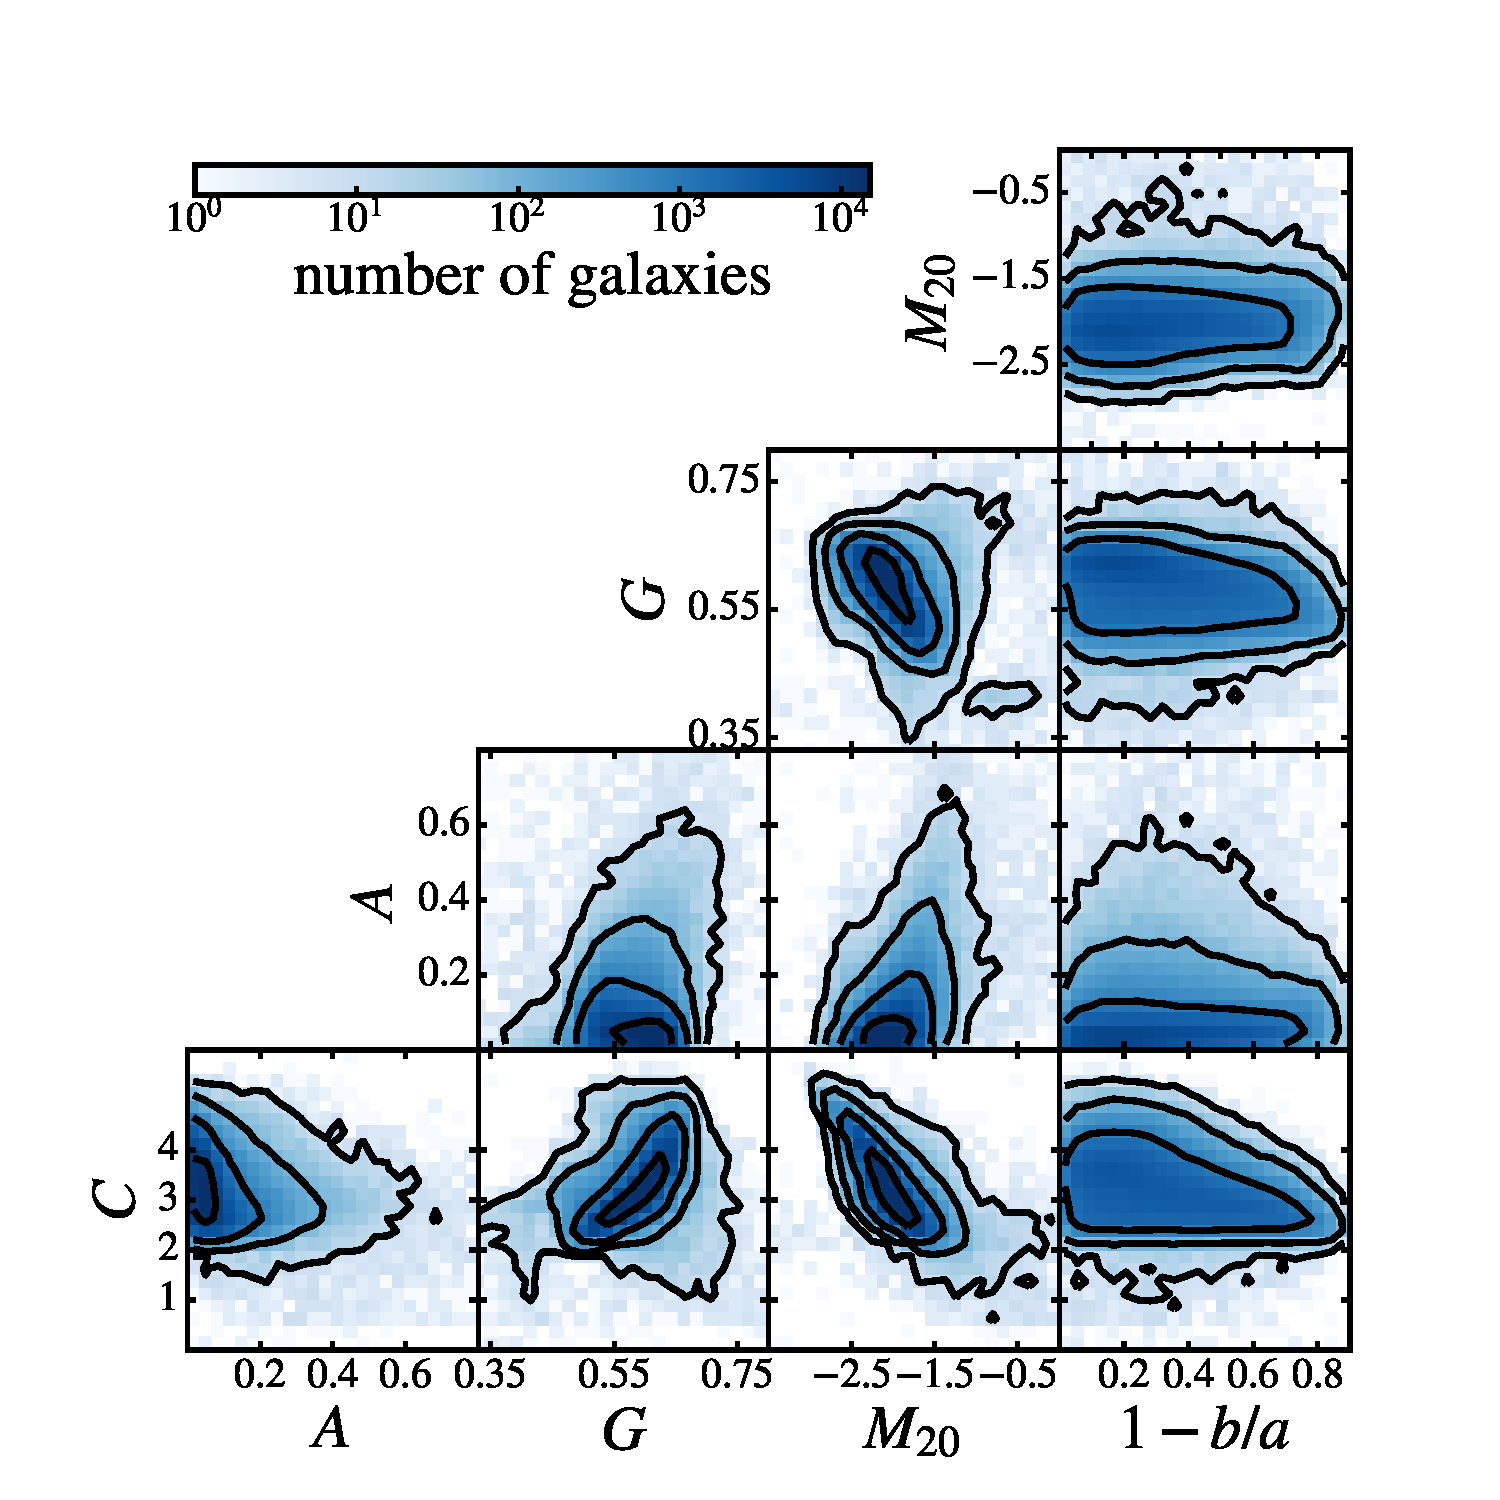
\includegraphics[width=3.7in]{figures/morph_params_entire_GZ2_sample.pdf}
\caption{\textit{Left.} Identifying~\feat~subjects is independent of identifying~\notfeat~subjects.  Both ROC curves use all subjects processed by SWAP where the score used to create the ROC curve is simply each subject's achieved posterior probability. The Featured curve demonstrates how well we identify~\feat~subjects with a threshold of 0.99, while the Not Featured curve demonstrates how well we identify~\notfeat~subjects with a threshold of 0.004. Typically, best performance is achieved by the score associated with the upper-left-most part of the curve. Our~\feat~threshold is nearly optimal, while our~\notfeat~threshold could be improved since the blue square is not as close to the upper left hand corner as other possible values of the subject posterior. \textit{Right.} Relation between measured morphology diagnostics for more than 280K SDSS galaxies. Most of these galaxies are processed through SWAP, receiving a posterior probability that estimates how likely each is to be~\feat~or~\notfeat.}
\label{fig: morph thresh}
\end{figure*}


\textbf{Subject prior probability,~\p.}
The prior probability assigned to each subject is an educated guess of 
the frequency of that characteristic in the scope of the data at hand. 
For galaxy morphologies, this number should be an estimate of the probability
of observing a desired feature (bar, disk, ring, etc.). In our case, 
we desire simply to find galaxies that are~\feat; however, this is dependent 
on mass, redshift, physical size, etc. The original GZ2 sample was selected
primarily on magnitude and redshift.  As there was no cut on galaxy size
(with the exception that each galaxy be larger than the SDSS PSF), the sample
includes a large range of  masses and sizes. Designating a single prior is not clear-cut; 
we thus explore how various~\p~values effect the SWAP outcome.

We run simulations allowing~\p~to take values 0.2, 0.35, and 0.8 
and compare these to the fiducial run, with everything else remaining constant.
The results are shown in the right panels of Figure~\ref{fig: tweak swap}. 
We again find that SWAP is consistent in terms of subject retirement which varies by only 1\%. 
However, as can be seen in the top panel, the variation in our quality metrics is 
more pronounced. 
Firstly, though we retire nearly the same number of subjects over the course
of each simulation, they are less consistent than our previous runs. That is, 
only 95\% of retired subjects are common to all simulations. Secondly, of those that are 
common, only 94\% receive the same label from SWAP indicating that changing the prior 
is more likely to produce a different label for a given subject than changing the initial 
agent confusion matrix. Finally, there is also a larger spread for the day on which a subject 
is retired as compared to the fiducial run. These trends all contribute to a broader 
spread in accuracy, completeness, and purity as a function of project time.
We stress, however, that although more substantial than the previous comparison, 
these variations are all within $\pm5\%$. 

We can understand these variations more intuitively by considering the following.
Recall that our retirement thresholds,~\tf~and~\tn, have not changed in these simulations. 
When~\p~is small, the subject's probability is already closer to~\tn~in probability space, 
and thus more subjects are classified as~\notfeat~compared to the fiducial run.
Similarly, when~\p~is large, some of these same subjects can instead be classified
as~\feat~because~\p~is already closer to~\tf. Obviously, both outcomes cannot be correct. 
We find that the simulation with~\p~= 0.8 performs the worst of any run; 
this is a direct reflection of the fact that this prior is not suitable for this question or this dataset. 
 Indeed, the best performance is achieved when~\p = 0.35.  This reflects the 
distribution of~\feat~subjects as determined by~\raw~labels and is more characteristic
of the expected proportion of~\feat~galaxies in the local universe.
As a value far from the correct value can have a significant impact on the classification
quality, it is important to choose a prior wisely.
 


\textbf{Retirement thresholds, \tf~and~\tn.}
Retirement thresholds are directly related to the time that a subject will spend
in SWAP before retirement.  If we lower~\tf~(and/or raise~\tn), more subjects will be retired
compared to the fiducial run as each subject will have a smaller swath of probability space
in which to fluctuate before crossing one of these thresholds.
On the other hand, if we raise~\tf~(and/or lower~\tn), it will take longer for subjects
to cross one of these thresholds. This also increases the likelihood of some subjects 
never crossing either threshold, instead oscillating indefinitely through probability space.

What thresholds should one choose? To answer this question, we consider the left panel of
Figure~\ref{fig: morph thresh}, which depicts the receiver operating 
characteristic (ROC) curve for our fiducial simulation, an illustration of performance as a 
function of a threshold for a binary classifier. 
ROC curves display the true positive rate against the false positive rate for 
a discriminatory threshold or score with a perfect classifier achieving 100\% true positives
and no false positives. The value of the threshold optimal for predicting class labels would 
be that which allows the ROC curve to reach the upper-left-most point in the diagram. 
We have two thresholds to consider and thus we plot the curve twice: 
once under the assumption that ``true positives" denote correctly identified~\feat~subjects; 
and again under the assumption that ``true positives" instead denote correctly identified~\notfeat~subjects.  In both cases, the color of the line corresponds to the 
subject posterior probability. We mark the location of~\tf~$=0.99$~and~\tn~$=0.004$
from our fiducial run with a red triangle and blue square respectively. 
 We see that~\tf~is nearly optimal but~\tn~could be improved upon. 



%% ----------------------------------------------------------------------------------------------------------------------------------------------
%% 		MEASURING MORPH PARAMS ON SDSS STAMPS
%% ----------------------------------------------------------------------------------------------------------------------------------------------
\section{Measuring Nonparametric Morphological Diagnostics on SDSS Stamps}
\label{sec: measuring morphology}

In order to train our Random Forest machine learning algorithm, we measure  non-parametric
morphology diagnostics for the GZ2 galaxy sample. 

We obtain $i$-band imaging from SDSS Data Release 12. Postage stamps are made from the SDSS fields for each galaxy with dimensions of 3 Petrosian radii. Galaxies located within 3 Petrosian radii of the edge of a field were excluded.  Postage stamps undergo a cleaning process whereby nearby sources are identified with SExtractor \citep[ver. 2.8.6;][]{sextractor} and their pixels replaced with values that mimic the background in that region. We compute the following widely adopted nonparametric measurements  of the galaxy light distribution on the cleaned postage stamps:


Concentration is computed as $C = 5\log(r_{80}/ r_{20})$ where \rr{80} and \rr{20} are the radii containing 80\% and 20\% of the galaxy light respectively.  Small values of this ratio tend to indicate disky galaxies, while larger values correlate with early-type ellipticals. 

Asymmetry quantifies the degree of rotational symmetry in the galaxy light distribution (not necessarily the physical shape of the galaxy as this parameter is not highly sensitive to low surface brightness features). A correction for background noise is applied (as in e.g.~\cite{Conselice2000}), i.e., 
\begin{equation}
A = \frac{\sum_{x,y} |I - I_{180}|}{ 2\sum|I|} - B_{180}
\end{equation}
where $I$ is the galaxy flux in each pixel $(x, y)$, $I_{180}$ is the image rotated by 180 degrees about the galaxy's central pixel, and $B_{180}$ is the average asymmetry of the background. 

The Gini coefficient, $G$,~\citep{Glasser1962, Abraham2003} describes how uniformly distributed a galaxy's flux is.  If $G$ is 0, the flux is distributed homogeneously among all galaxy pixels.; if $G$ is 1,  the light is contained within a single pixel. This term correlates with $C$, however, $G$ does not require that the flux be in the central region of the galaxy.  We follow~\cite{Lotz2004} by first ordering the pixels by increasing flux value, and then computing
\begin{equation}
G = \frac{1}{|\bar X|n(n-1)}\sum_i^n(2i-n-1)|X_i|
\end{equation}
where $n$ is the number of pixels assigned to the galaxy, and $\bar X$ is the mean pixel value. 

\M{20}~\citep{Lotz2004} is the second order moment of the brightest 20\% of the galaxy flux. We compute it as
\begin{eqnarray}
 M_{tot} & = & \sum_i^nf_i[(x_i-x_c)^2 + (y_i-y_c)^2]  \\
 M_{20} & = & \log_{10} (\frac{\sum_iM_i}{M_{tot}}), ~~\textrm{while} \sum_ifi < 0.2f_{tot}
\end{eqnarray}
where M$_{tot}$, the total moment, is computed first and $f_{tot}$ is the total flux. For centrally concentrated objects, \M{20} correlates with $C$ but is also sensitive to bright off-center knots of light. 

Finally, we use the ellipticity, $\epsilon = 1 - b/a$, of the light distribution as measured by SExtractor which computes the semi-major axis $a$ and semi-minor axis $b$ from the second-order moments of the galaxy light.  

In total, we measure morphological indicators for 282,350 SDSS galaxies. The relations between these diagnostics for the full sample is shown in the right panel of Figure~\ref{fig: morph thresh}. The code developed to clean and compute these morphology indicators is open source and can be found at \url{https://github.com/melaniebeck/measure_morphology}.





%% The reference list follows the main body and any appendices.
%% Use LaTeX's thebibliography environment to mark up your reference list.
%% Note \begin{thebibliography} is followed by an empty set of
%% curly braces.  If you forget this, LaTeX will generate the error
%% "Perhaps a missing \item?".
%%
%% thebibliography produces citations in the text using \bibitem-\cite
%% cross-referencing. Each reference is preceded by a
%% \bibitem command that defines in curly braces the KEY that corresponds
%% to the KEY in the \cite commands (see the first section above).
%% Make sure that you provide a unique KEY for every \bibitem or else the
%% paper will not LaTeX. The square brackets should contain
%% the citation text that LaTeX will insert in
%% place of the \cite commands.

%% We have used macros to produce journal name abbreviations.
%% \aastex provides a number of these for the more frequently-cited journals.
%% See the Author Guide for a list of them.

%% Note that the style of the \bibitem labels (in []) is slightly
%% different from previous examples.  The natbib system solves a host
%% of citation expression problems, but it is necessary to clearly
%% delimit the year from the author name used in the citation.
%% See the natbib documentation for more details and options.


\bibliographystyle{apj}
\bibliography{apj-jour,human-machine}

%% This command is needed to show the entire author+affilation list when
%% the collaboration and author truncation commands are used.  It has to
%% go at the end of the manuscript.
%\allauthors

%% Include this line if you are using the \added, \replaced, \deleted
%% commands to see a summary list of all changes at the end of the article.
\listofchanges

\end{document}

%% End of file `sample.tex'.